% \documentclass[sigconf]{acmart}
\documentclass[sigconf,review]{acmart}\settopmatter{printfolios=true}

\usepackage{amssymb}
\usepackage{amsthm}
\usepackage{graphicx}
\usepackage{amsmath}
\usepackage{mathptmx}
\usepackage{mathtools}
\usepackage{stmaryrd}
\usepackage{adjustbox}
\usepackage{hyperref}
\usepackage{alltt}
\usepackage{url}
\usepackage{float}
\usepackage{minipage-marginpar}
\usepackage{style/utils}
\usepackage{style/code}
\usepackage{style/proof}
\usepackage{style/keywords}
\usepackage{style/layout}
\usepackage{style/judgements}

% for combinator pictures
\usepackage{tikz}
\usepackage{pgfplots}
\usetikzlibrary{shapes,arrows}

%\setcopyright{none}
\bibliographystyle{ACM-Reference-Format}
% \citestyle{acmauthoryear}

% -----------------------------------------------------------------------------
\begin{document}

\copyrightyear{2017}
\acmYear{2017}
\setcopyright{acmlicensed}
\acmConference{PPDP'17}{October 9--11, 2017}{Namur, Belgium}\acmPrice{15.00}\acmDOI{10.1145/3131851.3131865}
\acmISBN{978-1-4503-5291-8/17/10}

\begin{CCSXML}
<ccs2012>
<concept>
<concept_id>10003752.10003753.10003760</concept_id>
<concept_desc>Theory of computation~Streaming models</concept_desc>
<concept_significance>500</concept_significance>
</concept>
</ccs2012>
\end{CCSXML}


\renewcommand{\textrightarrow}{$\rightarrow$}

\ccsdesc[500]{Theory of computation~Streaming models}


\title{Machine Fusion}
\subtitle{Merging merges, more or less}

\author{Amos Robinson}
\affiliation{Ambiata and UNSW (Australia)}
\email{amosr@cse.unsw.edu.au}

\author{Ben Lippmeier}
\affiliation{Digital Asset and UNSW (Australia)}
\email{benl@ouroborus.net}

\makeatactive
\begin{abstract}
Compilers for stream programs often rely on a fusion transformation to convert the implied dataflow network into low-level iteration based code. Different fusion transformations handle different sorts of networks, with the distinguishing criteria being whether the network may contain splits and joins, and whether the set of fusible operators can be extended. We present the first fusion system that simultaneously satisfies all three of these criteria: networks can contain splits, joins, and new operators can be added to the system without needing to modify the overall fusion transformation.
\end{abstract}

\maketitle


\section{Introdution}

This is some stuff.

%!TEX root = ../Main.tex

% -----------------------------------------------------------------------------
\section{Processes and Machines}
\label{s:Processes}

A \emph{process} in our system is a simple imperative program with a local heap. A process pulls source values from an arbitrary number of input streams and pushes result values to at least one output stream. The process language is an intermediate representation we use when fusing the overall dataflow network. When describing the fusion transform we describe the control flow of the process as a state machine, hence Machine Fusion. 

A \emph{combinator} is a template for a process which parameterizes it over the particular input and output streams, as well as values of configuration parameters such as the worker function used in a @map@ process. Each process implements a logical \emph{operator} --- so we use ``operator'' when describing the values being computed, but ``process'' and ``machine'' when referring to the implementation. 


% -----------------------------------------------------------------------------
\subsection{Grouping}

The definition of the @group@ combinator which detects groups of successive identical elements in the input stream is given in Figure~\ref{fig:Process:Group}. The process emits the first value pulled from the stream and every value that is different from the last one that was pulled. For example, when executed on the input stream @[1,2,2,3]@, the process will produce the output @[1,2,3]@. We include the concrete representation and a diagram of the process when viewed as a state machine.

The @group@ combinator has two parameters, @sIn1@ and @sOut1@, which bind the input and output streams respectively. The \emph{nu-binders} \mbox{($\nu$ @(f: Bool) (l: Nat)@...)} indicate that each time the @group@ combinator is instantiated, fresh names must be given to @f@, @l@ and so on, that do not conflict with other instantiations. Overall, the @f@ variable tracks whether we are dealing with the first value from the stream, @l@ holds the last value pulled from the stream (or 0 if none have been read yet), and @v@ holds the current value pulled from the stream. 

The body of the combinator is a record that defines the process. The @ins@ field defines the set of input streams and the @outs@ field the set of output streams. The @heap@ field gives the initial values of each of the local variables. The @instrs@ field contains a set of labeled instructions that define the program, while the @label@ field gives the label of the initial instruction. In this form, the output stream is defined via a parameter, rather than being the result of the combinator, as in the representation of @uniquesUnion@ from \S\ref{s:Introduction}. 

The initial instruction @(pull sIn1 v A1 [])@ pulls the next element from the stream @sIn1@, writes it into the heap variable @v@ (value), then proceeds to the instruction at label @A1@. The empty list @[]@ after the target label @A1@ can be used to update heap variables, but as we do not need to update anything yet we leave it empty. 

Next, the instruction @(case (f || (l /= v)) A2 [] A3 [])@ checks whether predicate @(f || (l /= v))@ is true; if so it proceeds to the instruction at label @A2@, otherwise it proceeds to @A3@. We use the variable @l@ (last) to track the last value read from the stream, and the boolean @f@ (first) to track whether this is the first element.

% AR: Clumsy, but added "at L2 executes:" to force @(push...)@ onto its own line. Otherwise it goes off the right.
When the predicate is true, the instruction at label @A2@ executes
@(push sOut1 v A3 [ l = v, f = F ])@
which pushes the value @v@ to the output stream @sOut1@ and proceeds to the instruction at label @A3@, once the variable @l@ is set to @v@ and @f@ to @F@ (False).

Finally, the instruction @(drop sIn1 A0 [])@ signals that the current element that was pulled from stream @sIn1@ is no longer required, and goes back to the first instruction at @A0@. 


\begin{figure*}

\begin{minipage}{0.6\textwidth}
\begin{alltt}
 group 
   = \(\lambda\) (sIn1: Stream Nat) (sOut1: Stream Nat). 
     \(\nu\) (f: Bool) (l: Nat) (v: Nat) (A0..A3: Label).
\end{alltt}
\begin{code}
     process
      { ins:    { sIn1  }
      , outs:   { sOut1 }
      , heap:   { f = T, l = 0, v = 0 }
      , label:  A0
      , instrs: { A0 = pull sIn1 v          A1 []
                , A1 = case (f || (l /= v)) A2 []  A3 []
                , A2 = push sOut1 v         A3 [ l = v, f = F ]
                , A3 = drop sIn1            A0 [] } }
\end{code}
\end{minipage}
\begin{minipage}{0.29\textwidth}
\includegraphics[scale=1.0]{figures/state-group.pdf}
\end{minipage}

\caption{The group combinator}
\label{fig:Process:Group}
\end{figure*}


% -----------------------------------------------------------------------------
\subsection{Merging}
\begin{figure*}
\begin{alltt}
       merge
         = \(\lambda\) (sIn1: Stream Nat) (sIn2: Stream Nat) (sOut2: Stream Nat). 
           \(\nu\) (x1: Nat) (x2: Nat) (B0..E2: Label).
\end{alltt}
\begin{code}
           process
            { ins:    { sIn1, sIn2 }
            , outs:   { sOut2 }
            , heap:   { x1 = 0, x2 = 0 }
            , label:  B0
            , instrs: { B0 = pull sIn1  x1   B1 []             , B1 = pull sIn2  x2   C0 []
                      , C0 = case (x1 < x2)  D0 []  E0 []      , D0 = push sOut2 x1   D1 []
                      , D1 = drop sIn1       D2 []             , D2 = pull sIn1  x1   C0 []
                      , E0 = push sOut2 x2   E1 []             , E1 = drop sIn2       E2 []
                      , E2 = pull sIn2 x2    C0 [] } }
\end{code}
\includegraphics[scale=1.0]{figures/state-merge.pdf}
\caption{The merge combinator}
\label{fig:Process:Merge}
\end{figure*}

The definition of the @merge@ combinator, which merges two input streams, is given in Figure~\ref{fig:Process:Merge}. The combinator binds the two input streams to @sIn1@ and @sIn2@, while the output stream is @sOut2@. The two heap variables @x1@ and @x2@ store the last values read from each input stream. The process starts by pulling from each of the input streams. It then compares the two pulled values, and pushes the smaller of the values to the output stream. The process then drops the stream which yielded the the smaller value, then pulls from the same stream so that it can perform the comparison again.


% -----------------------------------------------------------------------------
\subsection{Fusion}

Our fusion algorithm takes two processes and produces a new one that computes the output of both. For example, suppose we need a single process that produces the output of the first two lines of our @uniquesUnion@ example back in \S\ref{s:Introduction}. The result will be a process that computes the result of both @group@ and @merge@ as if they were executed concurrently, where the first input stream of the @merge@ process is the same as the input stream of the @group@ process. In our informal description of the fusion algorithm we will instantiate the parameters of each combinator with arguments of the same names.

% -----------------------------------------------------------------------------
\subsubsection{Fusing Pulls}
\label{s:Fusion:FusingPulls}

The algorithm proceeds by considering pairs of states: one from each of the source process state machines to be fused. Both the @group@ machine and the @merge@ machine pull from the same stream as their initial instruction, so we have the situation shown in the top of Figure~\ref{fig:Fusion:Pulls}. The @group@ machine needs to transition from label @A0@ to label @A1@, and the @merge@ machine from @B0@ to @B1@. In the result machine we produce three new instructions that transition between four joint result states, @F0@ to @F3@.
Each of the joint result states represents a combination of two source states, one from each of the source machines. For example, the first result state @F0@ represents a combination of the @group@ machine being in its initial state @A0@ and the @merge@ machine being in its own initial state @B0@. 

We also associate each of the joint result states with a description of whether each source machine has already pulled a value from each of its input streams. For the @F0@ case at the top of Figure~\ref{fig:Fusion:Pulls} we have ((A0, \{sIn1 = none\}), (B0, \{sIn1 = none, sIn2 = none\})). The result state @F0@ represents a combination of the two source states @A0@ and @B0@. As both @A0@ and @B0@ are the initial states of their respective machines, those machines have not yet pulled any values from their two input streams, so both `sIn1' and `sIn2' map to `none'.

From the result state @F0@, both of the source machines then need to pull from stream @sIn1@, the @group@ machine storing the value in a variable @v@ and the @merge@ machine storing it in @x1@. In the result machine this is managed by first storing the pulled value in a fresh, shared buffer variable @b1@, and then using later instructions to copy the value into the original variables @v@ and @x1@. To perform the copies we attach updates to a @jump@ instruction, which otherwise transitions between states without affecting any of the input or output streams.

Finally, note that in the result states @F0@ through @F3@, the state of the input streams transitions from `none', to `pending' then to `have'. The `none' state means that we have not yet pulled a value from the associated stream. The `pending' state means we have pulled a value into the stream buffer variable (@b1@ in this case). The `have' state means that we have copied the pulled value from the stream buffer variable into the local variable used by each machine. 

% BL: Dropped this to fix pagination.
% In Figure~\ref{fig:Fusion:Pulls},  `sIn1' is set to `have' for the first machine in @F2@ after we have set `v = b1', while `sIn1' is set to `have' for the second machine in @F3@ after we have set `x1 = b1'. 


% -----------------------------------------------------------------------------
\subsubsection{Fusing Cases}
Once the result machine has arrived at the joint state @F3@, this is equivalent to the two source machines arriving in states @A1@ and @B1@ respectively. The lower half of Figure~\ref{fig:Fusion:Case} shows the next few transitions of the source machines. From state @A1@, the @group@ machine needs to perform a @case@ branch to determine whether to push the current value it has from its input stream @sIn1@ to output stream @sOut1@, or to just pull the next value from its input. From state @B1@, the @merge@ machine needs to pull a value from its second input stream @sIn2@. In the result machine, @F3@ performs the case analysis from @A1@, moving to either @F4@ or @F5@, corresponding to @A2@ and @A3@ respectively. From state @F4@, the push at @A2@ is executed and moves to @F5@, corresponding to @A3@. Finally, at @F5@ the @merge@ machine pulls from @sIn2@, moving from @F5@ to @F6@, corresponding to @B1@ and @C0@ respectively. As the stream @sIn2@ is only pulled from by the @merge@ machine, no coordination is required between the @merge@ and @group@ machines for this pull.


% -----------------------------------------------------------------------------
\subsection{Fused Result}

Figure~\ref{fig:Process:Fused} shows the final result of fusing @group@ and @merge@ together. There are similar rules for handling the other combinations of instructions, but we defer the details to \S\ref{s:Fusion}. The result process has two input streams, @sIn1@ and @sIn2@, and two output streams: @sOut1@ from @group@, and @sOut2@ from @merge@. The shared input @sIn1@ is pulled by @merge@ instructions at two places, and since both of these need to agree with when @group@ pulls, the @group@ instructions are duplicated at @F3@-@F5@ and @F13@-@F15@. The first set of instructions could be simplified by constant propagation to a single @push@, as @f@ is initially true.

To complete the implementation of our example from \S\ref{s:Introduction} we would now fuse this result process with a process from the final line of the example (also a @group@). Note that although the result process has a single shared heap, the heap bindings from each fused process are guaranteed not to interfere, as when we instantiate combinators to create source processes we introduce fresh names. 

% AR: Cut to make room for explanation why two copies of group pull
% The order in which pairs of processes are fused together does matter, as does the order in which instructions are interleaved --- we discuss both points further in \S\ref{s:FusionOrder} and \S\ref{s:Evaluation}.

% -----------------------------------------------------------------------------
\subsection{Breaking It Down}
We started with a pure functional program in \S\ref{s:Introduction}, reimagined it as a dataflow graph, then interleaved imperative code that implemented two of the operators in that dataflow graph. We needed to \emph{break down} the definition of each operator into imperative statements so that we could interleave their execution appropriately. We do this because the standard, single-threaded evaluation semantics of functional programs does not allow us to evaluate stream programs that contain both splits and joins in a space efficient way. Returning to the definition of @uniquesUnion@ from \S\ref{s:Introduction}, we cannot simply execute the @group@ operator on its entire input @sIn1@ before executing the @merge@ operator, as that would require us to buffer all data read from @sIn1@. Instead, during fusion we perform the job of a concurrent scheduler at compile time. In the result process the flow of control alternates between the instructions for both the @group@ and @merge@ operators, but as the instructions are interleaved directly there is no overhead due to context switching --- as there would be in a standard concurrent implementation using multiple threads.

The general approach of converting a pure functional program to a dataflow graph, then interleaving imperative statements that implement each operator was also used in prior work on Flow Fusion~\cite{lippmeier2013data}. However, in contrast to Flow Fusion and similar systems, with \mbox{Machine Fusion} we do not need to organize statements into a fixed \emph{loop anatomy} --- we simply merge them as they are. This allows us to implement a wider range of operators, including ones with nested loops that work on segmented streams.

Note that relying on lazy evaluation for @uniquesUnion@ does not eliminate the need for unbounded buffering. Suppose we converted each of the streams to lazy lists, and used definitions of @group@ and @merge@ that worked over these lists. As @uniquesUnion@ returns a pair of results, there is nothing preventing a consumer from demanding the first list (@sUnique@) in its entirety before demanding any of the elements from the second list (@sUnion@). If this were to happen then the runtime implementation would need to retain all elements of @sIn1@ before demanding any of @sIn2@, causing a space leak. Lazy evaluation is \emph{pull only} meaning that evaluation is driven by the consumer. The space efficiency of our fused program relies critically on the fact that processes can also \emph{push} their result values directly to their consumers, and that the consumers cannot defer the handling of these values.

% TODO: Blend this in.
% Note that we could construct the fused result machine in several ways. One option is to perform the case branch first and then pull from @sIn2@, another is to pull from @sIn2@ first and then perform the branch. By construction, the predicate used in the branch refers only to variables local to the @group@ machine, and the pull instruction from @B1@ stores its result in a variable local to the @merge@ machine. As the set of variables does not overlap, either ordering is correct. For this example we choose to perform the branch first, though will discuss the ramifications of this choice further in \S\ref{s:FusionOrder}. 

% TODO: Shift this later.
% As the @merge@ process merges infinite streams, if we execute it with a finite input prefix, it will arrive at an intermediate state that may not yet have pushed all available output. For example, if we execute the process with the input streams @[1,4]@ and @[2,3,100]@ then the values @[1,2,3,4]@ will be pushed to the output. After pushing the last value @4@, the process will block at instruction @E2@, waiting for the next value to become available from @sIn2@. We discuss how to handle finite streams later in ~\S\ref{s:Finite}.

% TODO: Talk about what drop is really for later.
% This @drop@ instruction is used to coordinate concurrent processes when performing fusion. The next element of a stream may only be pulled after all consumers of that stream have pulled and then and dropped the current element.

% -----------------------------------------------------------------------------
\begin{figure*}
\includegraphics[scale=1.1]{figures/fuse-pull-pull.pdf}

\vspace{2em}

\includegraphics[scale=1.1]{figures/fuse-case-pull.pdf}
\caption{Fusing pull (top) and case (bottom) instructions}
\label{fig:Fusion:Pulls}
\label{fig:Fusion:Case}
\end{figure*}

% BL: Merged these figures togather to save space.
% \begin{figure*}
% \caption{Fusing case instructions}
% \label{fig:Fusion:Case}
% \end{figure*}

%%% AR: would like to highlight which machine is performing the current instruction, eg bolding "A0" when it's group moving from A0 to A1
\begin{figure*}
\definecolor{groupc}{HTML}{308030}
\definecolor{mergec}{HTML}{800000}
\definecolor{sharec}{HTML}{000080}

\newcommand\annot[5]{
  \tiny ((#1,   \> \tiny \{sIn1 =      #2\}), 
                \> \tiny (#3, \> \tiny \{sIn1 =      #4, \> \tiny sIn2 =      #5\}))
}

\newcommand\icase[7]{
 \tt{#1} \> \tt{= #2} \> \tt{#3} \> \tt{[ #4 ]} \> \tt{#5} \> \tt{[ #6 ]} \> \tiny #1 \> \tiny = #7
}

\newcommand\instr[5]{
 \tt{#1}\>\tt{= #2} \> \tt{#3} \> \tt{[ #4 ]} \> \> \> \tiny #1 \> \tiny = #5
}

\newcommand\tctt[2]{\textcolor{#1}{\tt{#2}}}

\hspace{5em}

\begin{adjustbox}{minipage=0.8\textwidth,margin=0pt \smallskipamount,center}
\begin{alltt}
process
\string{ ins:    \string{ \tctt{sharec}{sIn1},  \tctt{mergec}{sIn2} \string}
, outs:   \string{ \tctt{groupc}{sOut1}, \tctt{mergec}{sOut2} \string}
, heap:   \string{ \tctt{groupc}{f = T, l = 0, v = 0}, \tctt{mergec}{x1 = 0, x2 = 0}, \tctt{sharec}{b1 = 0} \string}
, label:  \tctt{sharec}{F0}
\end{alltt}

\begin{tabbing}
@  @ \=
@, F17@  \= = @case (f || (l /= v)) @
         \= @F17@ \= @[ ]     @ \= @F17@ \= @[ ]@
@   @ \= \tiny @   @F17 \= \tiny = ((A0, \= \tiny \{sIn1 = pending\}), \= \tiny (B0, \= \tiny \{sIn1 = pending, \= \tiny sIn2 = pending\})) \kill

@, instrs:@

% I have no idea how this works, but you need this particular incantation to colour the whole line in a tabbing environment.
% It's not ideal that the { and , are coloured too, but that can't be helped.
\\[0pt \color{sharec}]
\> @{@
\instr{F0}{pull sIn1 b1}{F1}{}
      {\annot{A0}{none}{B0}{none}{none}}

\\[0pt \color{groupc}]
\> @,@
\instr{F1}{jump}{F2}{v  = b1}
      {\annot{A0}{pending}{B0}{pending}{none}}

\\[0pt \color{mergec}]
\> @,@
\instr{F2}{jump}{F3}{x1 = b1}
      {\annot{A1}{have}{B0}{pending}{none}}

\\[0pt \color{groupc}]
\> @,@
\icase{F3}{case (f || (l /= v))}{F4}{}{F5}{}
      {\annot{A1}{have}{B1}{have}{none}}

\\[0pt \color{groupc}]
\> @,@
\instr{F4}{push sOut1 v}{F5}{l = v, f = F}
      {\annot{A2}{have}{B1}{have}{none}}

\\[0pt \color{groupc}]
\> @,@
\instr{F5}{jump}{F6}{}
      {\annot{A3}{have}{B1}{have}{none}}

\\[0pt \color{mergec}]
\> @,@
\instr{F6}{pull sIn2 x2}{F7}{}
      {\annot{A0}{none}{B1}{have}{none}}

\\
\\[0pt \color{mergec}]
\> @,@
\icase{F7}{case (x1 < x2)}{F8}{}{F16}{}
      {\annot{A0}{none}{C0}{have}{have}}

\\
\\[0pt \color{mergec}]
\> @,@
\instr{F8}{push sOut2 x1}{F9}{}
      {\annot{A0}{none}{D0}{have}{have}}

\\[0pt \color{mergec}]
\> @,@
\instr{F9}{drop sIn1}{F10}{}
      {\annot{A0}{none}{D1}{none}{have}}

\\[0pt \color{sharec}]
\> @,@
\instr{F10}{pull sIn1 b1}{F11}{}
      {\annot{A0}{none}{D2}{none}{have}}

\\[0pt \color{groupc}]
\> @,@
\instr{F11}{jump}{F12}{v = b1}
      {\annot{A0}{pending}{D2}{pending}{have}}

\\[0pt \color{mergec}]
\> @,@
\instr{F12}{jump}{F13}{x1 = b1}
      {\annot{A1}{have}{D2}{pending}{have}}

\\[0pt \color{groupc}]
\> @,@
\icase{F13}{case (f || (l /= v))}{F14}{}{F15}{}
      {\annot{A1}{have}{C0}{have}{have}}

\\[0pt \color{groupc}]
\> @,@
\instr{F14}{push sOut1 v}{F15}{l = v, f = F}
      {\annot{A2}{have}{C0}{have}{have}}

\\[0pt \color{groupc}]
\> @,@
\instr{F15}{jump}{F7}{}
      {\annot{A3}{have}{C0}{have}{have}}

\\

\\[0pt \color{mergec}]
\> @,@
\instr{F16}{push sOut2 x2}{F17}{}
      {\annot{A0}{none}{E0}{have}{have}}

\\[0pt \color{mergec}]
\> @,@
\instr{F17}{drop sIn2}{F18}{}
      {\annot{A0}{none}{E1}{have}{have}}

\\[0pt \color{mergec}]
\> @,@
\instr{F18}{pull sIn2}{F7}{}
      {\annot{A0}{none}{E2}{have}{none}}


\\[0pt \color{black}]
@} }@
\end{tabbing}
\end{adjustbox}
\caption{Fusion of \textcolor{groupc}{group} and \textcolor{mergec}{merge}, along with \textcolor{sharec}{shared} instructions}
\label{fig:Process:Fused}
\end{figure*}
% -----------------------------------------------------------------------------


%!TEX root = ../Main.tex

% -----------------------------------------------------------------------------
\section{Process definitions}
%!TEX root = ../Main.tex

\begin{figure*}
\begin{minipage}[t]{0.4\textwidth}
\begin{tabbing}
MMMMMx \TABDEF @MMMMM@  \TABSKIP $\Exp$ \TABSKIP $\Exp$ \TABSKIP $\Exp$ \kill

\Exp,~$e$       \> ::= \> ~~~ $x~|~v~|~e~e $ \\
                \> $\enskip|~$ \> ~~ $ (e~||~e) ~|~ e+e ~|~ e~@/=@~e ~|~ e < e$ \\
\Value,~$v$     \> ::= \> ~~~ $\mathbb{N}~|~\mathbb{B}~|~(\lambda{}x.~e)$ \\
\Heap,~$bs$     \> ::= \> ~~~ $\cdot~|~bs,~x~=~v$ \\
\Updates,~$us$  \> ::= \> ~~~ $\cdot~|~us,~x~=~e$
\\[0.5em]

\Proc,~$p$      \> ::=\> @process@ \\
MMMMMM \= M \= \kill
\> \> @ins:   @  $(\Chan ~\mapsto~ \InputState)$ \\
\> \> @outs:  @  $\sgl{\Chan}$ \\
\> \> @heap:  @  \Heap \\
\> \> @label: @  \Label \\
\> \> @instrs:@  $(\Label ~\mapsto~ \Instr)$ 
\\[0.5em]
\InputState \> ::= \> ~~ @none@~$|$~@pending@~\Value~$|$~@have@

\end{tabbing}
\end{minipage}
\begin{minipage}[t]{0.05\textwidth}
\quad
\end{minipage}
\begin{minipage}[t]{0.4\textwidth}
\begin{tabbing}
MMMMMM \TABDEF @MMMM@  \TABSKIP $\Chan$ \TABSKIP $\Chan$ \TABSKIP $\Exp$ \kill

\Var,~$x$       \> $\to$ \> ~~~ (value variable) \\
\Chan,~$c$      \> $\to$ \> ~~~ (channel name) \\
\Label,~$l$     \> $\to$ \> ~~~ (label name) \\ 
\ChannelStates  \> ~ =   \> ~~~ $(\Chan \mapsto \InputState)$ \\
\Action,~$a$   \> ::=    \> ~~~ $\cdot ~~|~~ \Push~\Chan~\Value$ \\[0.5em]

\Instr
    \> ::=\> @pull@  \> \Chan  \> \Var  \> \Next \\
    \TABALT  @push@  \> \Chan  \> \Exp  \> \Next \\
    \TABALT  @drop@  \> \Chan  \>       \> \Next \\
    \TABALT  @case@  \> \Exp   \> \Next \> \Next \\
    \TABALT  @jump@  \>        \>       \> \Next \\
\\[0.5em]

\Next \> = \> $\Label~\times~\Updates$ 
\end{tabbing}
\end{minipage}
\caption{Process definitions}
\label{fig:Process:Def}
\end{figure*}



The formal grammar for process definitions is given in Figure~\ref{fig:Process:Def}. Variables, Channels and Labels are specified by unique names. We refer to the \emph{endpoint} of a stream as a channel. A particular stream may flow into the input channels of several different processes, but can only be produced by a single output channel. For values and expressions we use an untyped lambda calculus with a few primitives chosen to facilitate the examples. The `$||$' operator is boolean-or, `+' addition, `/=' not-equal, and `$<$' less-than.

A $\Proc$ is a record with five fields: the @ins@ field specifies the input channels; the @outs@ field the output channels; the @heap@ field the process-local heap; the @label@ field the label of the instruction currently being executed, and the @instrs@ a map of labels to instructions. We use the same record when specifying both the definition of a particular process, as well as when giving the evaluation semantics. When specifying a process the @label@ field gives the entry-point to the process code, though during evaluation it is the label of the instruction currently being executed. Likewise, when specifying a process we usually only list channel names in the @ins@ field, though during evaluation they are also paired with their current $\InputState$. If an $\InputState$ is not specified we assume it is `none'. A network is a set of processes that are able to communicate with each other.

In the grammar of Figure~\ref{fig:Process:Def} the $\InputState$ has three options: @none@, which means no value is currently stored in the associated stream buffer variable, $(@pending@~\Value)$ which gives the current value in the stream buffer variable and indicates that it has not yet been copied into a process-local variable, and @have@ which means the pending value has been copied into a process-local variable. The $\Value$ attached to the @pending@ state is used when specifying the evaluation semantics of processes. When performing the fusion transform the $\Value$ itself will not be known, but we can still reason statically that a process must be in the @pending@ state. When defining the fusion transform in \S\ref{s:Fusion} we will use a version of $\InputState$ with only this statically known information.

The @instrs@ field of the $\Proc$ maps labels to instructions. The possible instructions are: @pull@, which pulls the next value from a channel into a given heap variable; @push@, which pushes the value of an expression to an output channel;  @drop@ which indicates that the current value pulled from a channel is no longer needed; @case@ which branches based on the result of a boolean expression, and @jump@ which causes control to move to a new instruction.

Instructions include a $\Next$ field containing the label of the next instruction to execute, as well as a list of $\Var \times \Exp$ bindings used to update the heap.
The list of update bindings is attached directly to instructions to make the fusion algorithm easier to specify, in contrast to a presentation with a separate @update@ instruction. 

When lowering process code to a target language, such as C, LLVM, or some sort of assembly code, we can safely convert @drop@ to plain @jump@ instructions. The @drop@ instructions are used to control how processes should be synchronized, but do not affect the execution of a single process. We discuss @drop@s further in \S\ref{s:Optimisation}.

% This allows us to \emph{deliberately} introduce artificial deadlocks when a process network would require more than one element of buffering.
%%% AR: added to highlight that this rules out networks that require unbounded buffers
%%% BL: We don't have any examples of explicitly introducing deadlocks. The process networks just happen to have them when viewed abstractly.

%%% AR: feels a bit disjointed because drops were only mentioned once a few paragraphs ago. Maybe reword to talk about lowering in general is obvious for most instructions, and drops are just treated as jumps. Or move up.


% -----------------------------------------------------------------------------
\subsection{Execution}
\label{s:Process:Eval}

The dynamic execution of a process network consists of:

\begin{enumerate}
\item \emph{Injection} of a single value from a stream into a process, or a network. Each individual process only needs to accept an injected  value when it is ready for it, and injection into a network succeeds only when they \emph{all} processes accept it.

\item \emph{Advancing} a single process from one state to another. Advancing a network succeeds when \emph{any} of the processes in the network can advance.

\item \emph{Feeding} outputs of some processes to the inputs of others. Feeding alternates between Injecting and Advancing. When a process pushes a value to an output channel we attempt to inject this value into all processes that have that same channel as an input. If they all accept it, we then advance their programs as far as they will go, which may cause more values to be pushed to output channels, and so on.
\end{enumerate}

Execution of a network is non-deterministic. At any moment several processes may be able to take a step, while others are blocked. As with Kahn processes~\cite{kahn1976coroutines}, pulling from a channel is blocking, which enables the overall sequence of values on each output channel to be deterministic. Unlike Kahn processes, pushing to a channel can also block. Each consumer has a single element buffer, and pushing only succeeds when that buffer is empty.

%%% AR: what is the distinction between 'execution' and 'evaluation'?  I only have a vague feeling that execution is something a computer does, while evaluation is the mathematical rules. Either way, these should probably be consistent.
%%% BL: "Evaluation" is pure.  E-"value"-ation. Execution has visible actions, like pushing to streams.

% TODO BL: Mention what happens if we choose a different ordering, 
% and how the particular ordering chosen is decided upon.
Importantly, it is the order in which values are \emph{pushed to each particular output channel} which is deterministic, whereas the order in which different processes execute their instructions is not. When we fuse two processes we choose one particular instruction ordering that enables the network to advance without requiring unbounded buffering. The single ordering is chosen by heuristically deciding which pair of states to merge during fusion, and is discussed in \S\ref{s:EvaluationOrder}.

Each channel may be pushed to by a single process only, so in a sense each output channel is owned by a single process. The only intra-process communication is via channels and streams. Our model is ``pure data flow'' as there are no side-channels between processes --- in contrast to ``impure data flow'' systems such as StreamIt~\cite{thies2002streamit}.


% -----------------------------------------------------------------------------
\subsubsection{Injection}
Figure~\ref{fig:Process:Eval:Inject} gives the rules for injecting values into processes. Injection is a meta-level operation, in contrast to @pull@ and @push@ which are instructions in the object language. The statement $(\ProcInject{p}{v}{c}{p'})$ reads ``given process $p$, injecting value $v$ into channel $c$ yields an updated process $p'$''. The @injects@ form is similar, operating on a process network.

Rule (InjectValue) injects a single value into a single process. The value is stored as a (@pending@~ v) binding in the $\InputState$ of the associated channel of the process. The $\InputState$ acts as a single element buffer, and must be empty (@none@) for injection to succeed.

Rule (InjectIgnore) allows processes that do not use a particular named channel to ignore values injected into that channel.

Rule (InjectMany) attempts to inject a single value into a network. We use the single process judgment form to inject the value into all processes, which must succeed for all of them.
% Once a value has been injected into all consuming processes that require it, the producing process no longer needs to retain it.

%!TEX root = ../Main.tex

\begin{figure*}
\begin{minipage}[t]{1\textwidth}

$$
\arrLR{
  \boxed{\ProcInject{\Proc}{\Value}{\Chan}{\Proc}}
}{
  \boxed{\ProcsInject{\sgl{\Proc}}{\Value}{\Chan}{\sgl{\Proc}}}
}
$$

$$
\ruleIN{
  p[@ins@][c] = @none@
}{
  \ProcInject{p}{v}{c}{p~[@ins@ \mapsto (p[@ins@][c \mapsto @pending@~v]) ] }
}{InjectValue}
$$

$$
\ruleIN{
  c \not\in p[@ins@]
}{
  \ProcInject{p}{v}{c}{p}
}{InjectIgnore}
%
\quad
%
\ruleIN{
  \{~ \ProcInject{p_i}{v}{c}{p'_i} ~\}^i
}{
  \ProcsInject{\sgl{p_i}^i}{v}{c}{\sgl{p'_i}^i}
}{InjectMany}
$$

\end{minipage}
\caption{Injection of values into input channels}
\label{fig:Process:Eval:Inject}
\end{figure*}



%!TEX root = ../Main.tex

% -----------------------------------------------------------------------------
\begin{figure*}
\begin{minipage}[t]{1\textwidth}

$$
  \boxed{
    \ProcBlockShake
      {\Instr}
      {\ChannelStates}
      {\Heap}
      {\Action}
      {\Label}
      {\ChannelStates}
      {\Updates}
  }
$$

$$
\ruleIN{
  is[c] = @pending@~v
}{
  \ProcBlockShake
        {@pull@~c~x~(l,us)}
        {is}
        {bs}
        {\cdot}
        {l}
        {is[c \mapsto @have@]}
        {(us, x = v)}
}{Pull}
%
\quad
%
\ruleIN{
  \ExpEval{bs}{e}{v}
}{
  \ProcBlockShake
        {@push@~c~e~(l,us)}
        {is}
        {bs}
        {\Push~c~v}
        {l}
        {is}
        {us}
}{Push}
$$

$$
\ruleIN{
  is[c] = @have@
}{
  \ProcBlockShake
        {@drop@~c~(l,us)}
        {is}
        {bs}
        {\cdot}
        {l}
        {is[c \mapsto @none@]}
        {us}
}{Drop}
\ruleIN{
}{
  \ProcBlockShake
        {@jump@~(l,us)}
        {is}
        {bs}
        {\cdot}
        {l}
        {is}
        {us}
}{Jump}
$$

$$
\ruleIN{
  \ExpEval{bs}{e}{@True@}
}{
  \ProcBlockShake
        {@case@~e~(l_t,us_t)~(l_f,us_f)}
        {is}
        {bs}
        {\cdot}
        {l_t}
        {is}
        {us_t}
}{CaseT}
\ruleIN{
  \ExpEval{bs}{e}{@False@}
}{
  \ProcBlockShake
        {@case@~e~(l_t,us_t)~(l_f,us_f)}
        {is}
        {bs}
        {\cdot}
        {l_f}
        {is}
        {us_f}
}{CaseF}
$$

\vspace{2em}

% ----------------
$$
  \boxed{\ProcShake{\Proc}{\Action}{\Proc}}
$$
$$
\ruleIN{
  \ProcBlockShake
    {p[@instrs@][p[@label@]]} 
    {p[@ins@]}
    {p[@heap@]}
    {a}
    {l}
    {is}
    {us}
  \quad
    \ExpEval{p[@heap@]}{us}{bs}
}{
  \ProcShake
        {p}
        {a}
        {p~[    @label@~ \mapsto ~l
           , ~~ @heap@~  \mapsto (p[@heap@] \lhd bs)
           , ~~ @ins@~   \mapsto ~is]}
}{Advance}
$$


\end{minipage}
\caption{Advancing processes}

% Evaluation: shaking allows proceses to take a step from one label to another as well as produce an output message. If the message is a push, the value is injected to all other processes in the network; otherwise it is an internal step.}
\label{fig:Process:Eval:Shake}
\end{figure*}


%!TEX root = ../Main.tex

\begin{figure*}
\begin{minipage}[t]{1\textwidth}

% ---------------------------------------------------------
$$
  \boxed{\ProcsShake{\sgl{\Proc}}{\Action}{\sgl{\Proc}}}
$$

$$
\ruleIN{
  \ProcShake{p_i}{\cdot}{p'_i}
}{
  \ProcsShake{
    \sgl{p_0 \ldots p_i \ldots p_n}
  }{\cdot}{
    \sgl{p_0 \ldots p'_i \ldots p_n}
  }
}{ProcessesInternal}
%
\quad
%
\ruleIN{
  \ProcShake{p_i}{\Push~c~v}{p'_i}
  \quad
  \forall j~|~j \neq i.~
  \ProcInject{p_j}{c}{v}{p'_j}
}{
  \ProcsShake{
    \sgl{p_0 \ldots p_i \ldots p_n}
  }{\Push~c~v}{
    \sgl{p'_0 \ldots p'_i \ldots p'_n}
  }
}{ProcessesPush}
$$


% ---------------------------------------------------------
\vspace{1em}

\newcommand\vs {\ti{vs}}
\newcommand\accs {\ti{accs}}
\newcommand\network {\ti{ps}}

$$
  \boxed{
    \ProcsFeed
      {(\Chan \mapsto \overline{Value})~}
      {\sgl{\Proc}}
      {(\Chan \mapsto \overline{Value})~}
      {\sgl{\Proc}}
  }
$$
$$
\ruleIN{
  \ProcsShake
    {ps}
    {\cdot}
    {ps'}
}{
  \ProcsFeed
    {cvs}
    {ps}
    {cvs}
    {ps'}
}{FeedInternal}
%
\quad
%
\ruleIN{
  \ProcsShake
    {ps}
    {\Push~c~v}
    {ps'}
}{
  \ProcsFeed
    {cvs}
    {ps}
    {cvs[c \mapsto (cvs[c] \listappend v)]}
    {ps'}
}{FeedPush}
$$


% $$
% \ruleIN{
%   (\forall p \in \network.~c \not\in @outs@~p)
% \quad
%   \ProcsFeed
%     {c=\vs, \accs}
%     {\network}
%     {\accs'}
%     {\network'}
% \quad
%   \ProcsInject
%     {\network'}
%     {c}{v}
%     {\network''}
% }{
%   \ProcsFeed
%     {c=\vs \listappend [v], \accs}
%     {\network}
%     {c=\vs \listappend [v], \accs'}
%     {\network''}
% }{FeedExternal}
% $$


$$
\ruleIN{
  (\forall p \in \network.~c \not\in p[@outs@])
\quad
  \ProcsInject
    {ps}
    {c}
    {v}
    {ps'}
}{
  \ProcsFeed
    {cvs[c \mapsto ([v] \listappend vs)]}
    {ps}
    {cvs[c \mapsto vs~]}
    {ps'}
}{FeedExternal}
$$



\end{minipage}
\caption{Feeding Process Networks}
\label{fig:Process:Eval:Feed}
\end{figure*}




% -----------------------------------------------------------------------------
\subsubsection{Advancing}
Figure~\ref{fig:Process:Eval:Shake} gives the rules for advancing a single process. The statement $(\ProcBlockShake{i}{is}{bs}{a}{l}{is'}{us'})$ reads ``instruction $i$, given channel states $is$ and the heap bindings $bs$, passes control to instruction at label $l$ and yields new channel states $is'$, heap update expressions $us'$, and performs an output action $a$.'' An output action $a$ is an optional message of the form $(\Push~\Chan~\Value)$, which encodes the value a process pushes to one of its output channels. We write ~$\cdot$~ for an empty action. 

Rule (Pull) takes the @pending@ value $v$ from the channel state and produces a heap update to copy this value into the variable $x$ in the @pull@ instruction. We use the syntax $us,x=v$ to mean that the list of updates $us$ is extended with the new binding $x=v$. In the result channel states, the state of the channel $c$ that was pulled from is set to @have@, to indicate the value has been copied into the local variable.

Rule (Push) evaluates the expression $e$ under heap bindings $bs$ to a value $v$, and produces a corresponding action which carries this value. The judgment $(bs \vdash e \Downarrow v)$ expresses standard untyped lambda calculus reduction using the heap $bs$ for the values of free variables. As this evaluation is completely standard we omit it to save space.

Rule (Drop) changes the input channel state from @have@ to @none@. A @drop@ instruction can only be executed after @pull@ has set the input channel state to @have@. 

Rule (Jump) produces a new label and associated update expressions. Rules (CaseT) and (CaseF) evaluate the scrutinee $e$ and emit the appropriate label.

The statement $\ProcShake{p}{a}{p'}$ reads ``process $p$ advances to new process $p'$, yielding action $a$''. Rule (Advance) advances a single process. We look up the current instruction for the process' @label@ and pass it, along with the channel states and heap, to the above single instruction judgment. The update expressions $us$ from the single instruction judgment are reduced to values before updating the heap. We use $(us \lhd bs)$ to replace bindings in $us$ with new ones from $bs$. As the update expressions are pure, the evaluation can be done in any order.


% -----------------------------------------------------------------------------
\subsubsection{Feeding}
Figure~\ref{fig:Process:Eval:Feed} gives the rules for collecting output actions and feeding the contained values to other processes. The first set of rules concerns feeding values to other processes within the same network, while the second exchanges input and output values with the environment the network is running in.

The statement $\ProcShake{ps}{a}{ps'}$ reads ``the network $ps$ advances to the network $ps'$ yielding output action $a$''.

Rule (ProcessInternal) allows an arbitrary process in the network to advance to a new state at any time, provided it does not yield an output action. This allows processes to perform internal computation.

% , without needing to synchronize with the rest of the network.

Rule (ProcessPush) allows an arbitrary process in the network to advance to a new state while yielding an output action $(@push@~c~v)$. For this to succeed it must be possible to inject the output value $v$ into all processes that have channel $c$ as one of their inputs.

% As all consuming processes must accept the output value at the time it is created, there is no need to buffer it further in the producing process. When any process in the network produces an output action we take that as the action of the whole network.

The statement $\ProcsFeed{cvs}{ps}{cvs'}{ps'}$ reads ``with channel values $cvs$, network $ps$ takes a step and produces new channel values $cvs'$ and network $ps'$''. The channel values $cvs$ map channel names to a list of values. For input channels of the overall network, we initialize the map to contain a list of input values for each channel. For output channels of the overall network, values pushed to those channels are also collected in the same channel map. In a concrete implementation the input and output values would be transported over some IO device, but for the semantics we describe the abstract behavior only.

Rule (FeedInternal) allows the network to perform local computation in the context of the channel values. 

Rule (FeedPush) collects an output action (@push@ $c$ $v$) produced by a network and appends the value $v$ to the list corresponding to the output channel $c$. 

Rule (FeedExternal) injects values from the external environment. This rule also has the side condition that values cannot be injected from the environment into output channels that are already owned by some process. This constraint is required for correctness proofs, but can be ensured by construction in a concrete implementation.
% The topology of the dataflow network does not change at runtime, so it only needs to be checked once, before execution.


% -----------------------------------------------------------------------------
\subsection{Non-deterministic Execution Order}
\label{s:EvaluationOrder}

The execution rules of Figure~\ref{fig:Process:Eval:Feed} are non-deterministic in several ways. Rule (ProcessInternal) allows any process to perform internal computation at any time, without synchronizing with other processes in the network; (ProcessPush) allows any process to perform a push action at any time, provided all other processes in the network are ready to accept the pushed value; (FeedExternal) also allows new values to be injected from the environment, provided all processes that use the channel are ready to accept the value.

In the semantics, allowing the execution order of processes to be non-deterministic is critical, as it defines a search space where we might find an order that does not require unbounded buffering. For a direct implementation of concurrent processes using message passing and operating system threads, an actual, working, execution order would be discovered dynamically at runtime. In contrast, the role of our fusion system is to construct one of these working orders statically. In the fused result process, the instructions will be scheduled so that they run in one of the orders that would have arisen if the network were executed dynamically. Fusion also eliminates the need to pass messages between processes --- once they are fused we can just copy values between heap locations.

% In our system, allowing the execution order of processes to be non-deterministic is critical, as it provides freedom to search for a valid ordering that does not require excessive buffering. Consider the following example, where the @alt2@ operator pulls two elements from its first input stream, then two from the second, before pushing all four to its output stream.
% \begin{code}
%   alternates : S Nat -> S Nat -> S Nat -> S (Nat, Nat)
%   alternates sInA sInB sInC
%    = let  s1   = alt2 sInA sInB
%           s2   = alt2 sInB sInC
%           sOut = zip s1 s2
%      in   sOut
% \end{code}
% 
% Note that the middle stream @sInB@ is shared, and the result streams from both @alt2@ operators are zipped into tuples. Given the inputs @sInA@ = @[a1,a2]@, @sInB@ = @[b1,b2]@ and @sInC@ = @[c1,c2]@ the output of @zip@ will be @[(a1,b1),(a2,b2),(b1,c1),(b2,c2)]@, assuming @a1,a2,b1,b2@ and so on are values of type @Nat@.
% 
% Now, note that the first @alt2@ process pushes values to its output stream @s1@ two at a time, and the second @alt2@ process also pushes values to its own output stream @s2@ two at a time. However, the downstream @zip@ process needs to pull one value from @s1@ then one from @s2@, then another from @s1@, then another from @s2@, alternating between the @s1@ and @s2@ streams. This will work, provided we can arrange for the two \emph{separate} @alt2@ processes to push to their separate output streams alternatively. They can still push two values at a time to their own outputs, but the downstream @zip@ process needs receive one from each process alternately. Here is a table of intermediate values to help make the explanation clearer:
% 
% \begin{code}
%     sInA = [a1, a2, a3, a4, a5 ...]
%     sInB = [b1, b2, b3, b4, b5 ...]
%     sInC = [c1, c2, c3, c4, c5 ...]
% 
%     s1   = alt2 sInA sInB 
%          = [a1, a2, b1, b2, a3, a4, b3, b4 ...]
% 
%     s2   = alt2 sInB sInC
%          = [b1, b2, c1, c2, b3, b4, c3, c4 ...]
% 
%     sOut = zip s1 s2
%          = [(a1,b1), (a2,b2), (b1,c1), (b2,c2) ...]
% \end{code}
% 
% Considering the last line in the above table, note that @zip@ needs to output a tuple of @a1@ and @b1@ together, then @a2@ and @b2@ together, and so on. The implementation of the @zip@ process will attempt to pull the first value @a1@ from stream @s1@, blocking until it gets it, then pull the next value @b1@ from stream @s2@, blocking until it gets it. While @zip@ is blocked waiting for @b1@, the first @alt2@ process cannot yet push @a2@. The execution order of the overall network is constrained by communication patterns of processes in that network.

% As we cannot encode all possible orderings into the definition of the processes themselves, we have defined the execution rules to admit many possible orderings. In a direct implementation of concurrent processes using message passing and operating system threads, an actual, working, execution order would be discovered dynamically at runtime. In contrast, the role of our fusion transform is to construct one of these working orders statically. In the fused result process, the instructions will be scheduled so that they run in one of the orders that would have arisen if the network was executed dynamically. In doing so, we also eliminate the need to pass messages between processes --- once they are fused we can just copy values between heap locations.

% Although alt2 produces output elems two at a time, the consumer zip need its input elements to arrive alternately. At evaluation time we need the results pushed to sA1 and sA2 in the sA1 sA2 sA1 sA2 order, not sA1 sA1 sA2 sA2. Writing the rules nondeterministically allows the elaborator to discover a usable order, if there is one. This also affects fusion, we don't want to commit to the wrong order too early. We shall see that if we fuse the two alt processes first fusion will not work. We need to start with zip so that the order in which input elems arrive is constrained. 


%!TEX root = ../acc-optim.tex
\section{Array fusion} % (fold)
\label{sec:fusion}

\begin{figure}
\flushright
\small(Before fusion)\qquad\\
\centering
\includegraphics[scale=0.175]{figs/fusion1.pdf}
\flushright
\small(After producer/producer fusion)\qquad\\
\centering
\includegraphics[scale=0.175]{figs/fusion2.pdf}
\flushright
\small(After consumer/producer fusion)\qquad\\
\centering
\includegraphics[scale=0.175]{figs/fusion3.pdf}
\caption{Produce/producer and consumer/producer fusion}
\label{fig:Fusion}
\end{figure}

Fusion in a massively data-parallel, embedded language for GPUs, such as Accelerate, requires a few uncommon considerations.

\paragraph{Parallelism.} While fusing parallel collective operations, we must be careful not to lose information essential to parallel execution. For example, \texttt{foldr/build} fusion \cite{Gill:1993de} is not applicable, because it produces sequential tail-recursive loops rather than massively parallel GPU kernels. Similarly, the \texttt{split/join} approach used in Data Parallel Haskell (DPH)~\cite{Keller:distributed-types} is not helpful, although fused operations are split into sequential and parallel subcomputations, as they assume an explicit parallel scheduler, which in DPH is written directly in Haskell. Accelerate compiles massively parallel array combinators to CUDA code via template skeleton instantiation, so any fusion system must preserve the combinator representation of the intermediate code. 

\paragraph{Sharing.} Existing fusion transforms rely on inlining to move producer and consumer expressions next to each other, which allows producer/consumer pairs to be detected. However, when let-bound variables are used multiple times in the body of an expression, unrestrained inlining can lead to duplication of work. Compilers such as GHC, handle this situation by only inlining the definitions of let-bound variables that have a single use site, or by relying on some heuristic about the size of the resulting code to decide what to inline \cite{PeytonJones:Inliner}. However, in typical Accelerate programs, each array is used at least twice: once to access the shape information and once to access the array data; so, we must handle at least this case separately.

\paragraph{Filtering.} General array fusion transforms must deal with filter-like operations, for which the size of the result structure depends on the \emph{value} of the input structure, as well as its size. Accelerate does not encode filtering as a primitive operation, so we do not need to consider it further.\footnote{@filter@ is easily implemented as a combination of the core primitives, and is provided as part of the library.}

\paragraph{Fusion at run-time.}
As the Accelerate language is embedded in Haskell, compilation of the Accelerate program happens at Haskell \emph{runtime} rather than when compiling the Haskell program. For this reason, optimisations applied to an Accelerate program contribute to its overall runtime, so we must be mindful of the cost of analysis and code transformation. On the flip-side, runtime optimisations can make use of information that is only available at runtime. 

\paragraph{Fusion on typed de Brujin terms.}
We fuse Accelerate programs by rewriting typed de Bruijn terms in a type preserving manner. However, maintaining type information adds complexity to the definitions and rules, which amounts to a partial proof of correctness checked by the type checker, but is not particularly exciting for the present exposition. Hence, in this section, we elide the steps necessary to maintain type information during fusion.

\begin{table*}
\begin{lstlisting}[escapechar={\%}]
%\makebox[\textwidth]{\rm\bf Producers}%
map         :: (Exp a -> Exp b) -> Acc (Array sh a) -> Acc (Array sh b)             %\rm map a function over an array%
zipWith     :: (Exp a -> Exp b -> Exp c) -> Acc (Array sh a) -> Acc (Array sh b)    %\rm apply funciton to\ldots%
            -> Acc (Array sh c)                                                     %\rm \ldots a pair of arrays%
backpermute :: Exp sh' -> (Exp sh' -> Exp sh) -> Acc (Array sh a)                   %\rm backwards permutation%
            -> Acc (Array sh' e)
replicate   :: Slice slix => Exp slix                                               %\rm extend array across\ldots%
            -> Acc (Array (SliceShape slix) e)                                      %\rm \ldots new dimensions%
            -> Acc (Array (FullShape  slix) e)
slice       :: Slice slix                                                           %\rm remove existing dimensions%
            => Acc (Array (FullShape  slix) e) -> Exp slix
            -> Acc (Array (SliceShape slix) e)
generate    :: Exp sh -> (Exp sh -> Exp a) -> Acc (Array sh a)                      %\rm array from index mapping%

%\makebox[\textwidth]{\rm\bf Consumers}%
fold        :: (Exp a -> Exp a -> Exp a) -> Exp a -> Acc (Array (sh:.Int) a)        %\rm tree reduction along\ldots%
            -> Acc (Array sh a)                                                     %\rm \ldots innermost dimension%
scan{l,r}   :: (Exp a -> Exp a -> Exp a) -> Exp a -> Acc (Vector a)                 %\rm left-to-right or right-to-left%
            -> Acc (Vector a)                                                       %\rm \ldots vector pre-scan%
permute     :: (Exp a -> Exp a -> Exp a) -> Acc (Array sh' a)                       %\rm forward permutation%
            -> (Exp sh -> Exp sh') -> Acc (Array sh a) -> Acc (Array sh' a)
stencil     :: Stencil sh a stencil => (stencil -> Exp b) -> Boundary a             %\rm map a function with local\ldots%
            -> Acc (Array sh a) -> Acc (Array sh b)                                 %\rm \ldots neighbourhood context%
\end{lstlisting}
\caption[Core Accelerate array operations]{Summary of Accelerate's core
    collective array operations, omitting \texttt{Shape} and \texttt{Elt}
    class constraints for brevity. In addition, there are other flavours of
    folds and scans as well as segmented versions of these.}
\label{tab:operations}
\end{table*}


% -----------------------------------------------------------------------------
\subsection{The Main Idea}
All collective operations in Accelerate are array-to-array transformations. Reductions, such as \texttt{fold}, which reduce an array to a single element, yield a singleton array rather than a scalar expression. Hence, we can partition array operations into two categories:
%
\begin{enumerate}
\item Operations where each element of the result array depends on at most one element of each input array. Multiple elements of the output array may depend on a single input array element, but all output elements can be computed independently. We refer to these operations as \textit{producers}.

\item Operations where each element of the result array depends on multiple elements of the input array. We call these functions \textit{consumers}, in spite of the fact that they also produce an array.
\end{enumerate}
%
Table~\ref{tab:operations} summarises the collective array operations that we support. In a parallel context, producers are more pleasant to deal with because independent element-wise operations have an obvious mapping to the GPU. Consumers are a different story, as we need to know exactly how the computations depend on each other to implement them efficiently. For example, a parallel fold (with an associative operator) can be implemented efficiently as a tree reduction, but a parallel scan requires two separate phases \cite{Sengupta:2007tc, Chatterjee:1990vj}. Unfortunately, this sort of information is obfuscated by most fusion techniques. To support the different properties of producers and consumers, our fusion transform is split into two distinct phases:
%
\begin{itemize}
\item \emph{Producer/producer:} fuse sequences of producers into a single producer. This is implemented as a source-to-source transformation on the AST.

\item \emph{Consumer/producer:} fuse producers followed by a consumer into the consumer. This happens during code generation, where we specialise the consumer skeleton with the producer code.
\end{itemize}
%
Separating fusion into these two phases reduces the complexity of the task, though there is also a drawback: as all collective operations in Accelerate output arrays, we might wish to use the output of a consumer as an input to a producer as in @map g . fold f z@. Here, the \texttt{map} operation could be fused into the \texttt{fold} by applying the function \texttt{g} to each element produced by the reduction before storing the final result in memory. This is useful, as Accelerate works on multidimensional arrays, so the result of a \texttt{fold} can be a large array rather than just a singleton array. Our approach currently does not fuse producer/consumer pairs, only consumer/producer and producer/producer combinations. 

Figure~\ref{fig:Fusion} illustrates how fusion affects the AST: blue boxes $p_1$ to $p_7$ represent producers, where $p_5$ is a producer like \texttt{zipWith} with two input arrays. The consumers are $c_1$ and $c_2$. Firstly, we fuse all producers, with the exception of $p_1$ whose result is used by both $c_1$ and $p_2$. Next, we plug the fused producers into consumers where possible. Again, $p_1$ is left as is. It would be straightforward to change our implementation such that it would fuse $p_1$ into both $p_2$ and $c_1$. This would duplicate the work of $p_1$ into both $p_2$ and $c_1$, which, despite reducing memory traffic, is not always advantageous. Our current implementation is conservative and never duplicates work; we plan to change this in future work as the restricted nature of Accelerate means that we can compute accurate cost estimates and make an informed decision. In contrast, producer/consumer fusion of $c_1$ into $p_4$ would require fundamental changes.


% -----------------------------------------------------------------------------
\subsection{Producer/producer fusion for parallel arrays}

The basic idea behind the representation of producer arrays in Accelerate is well known: simply represent an array by its shape and a function mapping indices to their corresponding values. We previously used it successfully to optimise purely functional array programs in Repa~\cite{Keller:Repa}, but it was also used by others~\cite{Claessen:obsidian-expressive}.

However, there are at least two reasons why it is not always beneficial to represent all array terms uniformly as functions. One is \emph{sharing}: we must be able to represent some terms as manifest arrays so that a delayed-by-default representation can not lead to arbitrary loss of sharing. This is a well known problem in Repa. The other consideration is \emph{efficiency}: since we are targeting an architecture designed for performance, we prefer more specific operations. An opaque indexing function is too general, conveying no information about the pattern in which the underlying array is accessed, and hence no opportunities for optimisation. We shall return to this point in Section~\ref{sec:benchmarks}, but already include a form of structured traversal over an array (@Step@) in the following definition:

% It is parametrised with the shape of the result array, a function which, given
% an index in the result array, returns an index into the manifest source array
% argument.
\begin{code}
  data DelayedAcc a where
    Done  :: Acc a
          -> DelayedAcc a

    Yield :: (Shape sh, Elt e)
          => Exp sh
          -> Fun (sh -> e)
          -> DelayedAcc (Array sh e)

    Step  :: (Shape sh, Shape sh', Elt e, Elt e')
          => Exp sh'
          -> Fun (sh' -> sh)
          -> Fun (e -> e')
          -> Idx (Array sh e)
          -> DelayedAcc (Array sh' e')
\end{code}
%
We have three constructors: \texttt{Done} injects a manifest array into the
type. \texttt{Yield} defines a delayed array in terms of its shape and a
function which maps indices to elements. The third constructor, \texttt{Step},
encodes a special case of the more general \texttt{Yield} that represents the
application of an index and/or value space transformation to the argument array.
The type \texttt{Fun (sh -> e)} is that of a term representing a scalar
function from shape to element type. The type \texttt{Idx (Array sh e)} is that of a de
Bruijn index representing an array valued variable. Representing the argument
array in this way means that both \texttt{Step} and \texttt{Yield} are
non-recursive in \texttt{Acc} terms, and so they can always be expressed as
scalar functions and embedded into consumers in the second phase of fusion.

We represent all array functions as constructors of the type \texttt{DelayedAcc}. Producer/producer fusion is achieved by tree contraction on the AST, merging sequences of producers into a single one. All array producing functions, such as \texttt{map} and \texttt{backpermute}, are expressed in terms of smart constructors for the \texttt{DelayedAcc} type. The smart constructors manage the integration with successive producers, as shown in the following definition of \texttt{mapD}, the delayed version of the \texttt{map} function:
%
\begin{code}
  mapD :: (Shape sh, Elt a, Elt b)
       => Fun (a -> b)
       -> DelayedAcc (Array sh a)
       -> DelayedAcc (Array sh b)
  mapD f (Step  sh p g v) = Step  sh p (f . g) v
  mapD f (Yield sh g)     = Yield sh   (f . g)
\end{code}
%
The function composition operator \texttt{(.)} is overloaded here to work on scalar function terms. With this definition we now have the well known fusion rule that reduces \texttt{mapD f . mapD g} sequences to \texttt{mapD (f . g)}. Similarly, the definition of delayed backpermute means that \mbox{\texttt{backpermuteD sh p (backpermuteD \_ q arr)}} reduces to \texttt{backpermute sh (q . p) arr}:
\begin{code}
backpermuteD
    :: (Shape sh, Shape sh', Elt e)
    => Exp        sh'
    -> Fun        (sh' -> sh)
    -> DelayedAcc (Array sh  e)
    -> DelayedAcc (Array sh' e)
backpermuteD sh' p acc = case acc of
  Step  _ ix f a  -> Step  sh' (ix . p) f a
  Yield _ f       -> Yield env sh' (f . p)
  Done  env a     -> Step  sh' p identity (toIdx a)
\end{code}
% \gck{Manuel: as discussed, we may have to put in the valuation. Does backpermute really add anything here anyway?}
Of course, combinations of maps with backpermutes also reduce to a single producer. %, albeit one that does not correspond to one of the Accelerate built-in array operations.

As desired, this approach also works on producers which\linebreak
take their input from multiple arrays. This is in contrast to\linebreak
\texttt{foldr/build}~\cite{Gill:1993de}, which
can fuse one of the input arguments, but not both. The definition of \texttt{zipWithD} considers 
all possible combinations of constructors (only some of which we list here) and can therefore fuse producers of both arguments:
%
\begin{code}
  zipWithD :: (Shape sh, Elt a, Elt b, Elt c)
           => Fun (a -> b -> c)
           -> DelayedAcc (Array sh a)
           -> DelayedAcc (Array sh b)
           -> DelayedAcc (Array sh c)
  zipWithD f (Yield sh1 g1) (Yield sh2 g2)
    = Yield (sh1 `intersect` sh2)
            (\sh -> f (g1 sh) (g2 sh))
  zipWithD f (Yield sh1 g1) (Step  sh2 ix2 g2 a2)
    = Yield ...
\end{code}
%
In this manner, sequences of producers fuse into a single producer term; then, we turn them back into a manifest array using the function \texttt{compute}. It inspects the argument terms of the delayed array to identify special cases, such as maps or backpermutes, as shown in the following snippet of pseudo-code:
%
\begin{code}
  compute :: DelayedAcc a -> Acc a
  compute (Done a)          = a
  compute (Yield sh f)      = Generate sh f
  compute (Step sh p f v)
    | sh == shape a, isId p, isId f 
                            = a
    | sh == shape a, isId p = Map f a
    | isId f                = Backpermute sh p a
    | otherwise             = Transform sh p f a
    where a = Avar v
\end{code}
%
Since we operate directly on the AST of the program, we can inspect function arguments and specialise the code accordingly. For example, \texttt{isId :: Fun (a->b) -> Bool} checks whether a function term corresponds to the term $\lambda x. x$. 


% -----------------------------------------------------------------------------
\subsection{Consumer/Producer Fusion}
Now that we have the story for producer/producer fusion, we discuss how to deal with consumers. We pass producers encoded in the @DelayedAcc@ representation as arguments to consumers, so that the consumers can compute the elements they need on-the-fly. Consumers themselves have no @DelayedAcc@ representation, however.

Consumers such as \texttt{stencil}, access elements of their argument array multiple times. These consumers are implemented carefully not to duplicate work. Indeed, even when the argument of such a consumer is a manifest array, the consumer should ensure that it caches already fetched elements, as GPUs impose a high performance penalty for repeated memory loads. Some consumers can be implemented more efficiently when given a producer expressed in terms of a function from a multi-dimensional array index to an element value. Other consumers prefer functions that map the flat linear index of the underling array to its value. Our consumer-friendly representation of delayed arrays therefore contains both versions: 
%
\begin{code}
data Embedded sh e
  =  (Shape sh, Elt e) 
  => DelayedArray { extent      :: Exp sh
                  , index       :: Fun (sh  -> e)
                  , linearIndex :: Fun (Int -> e) }

embedAcc :: (Shape sh, Elt e) 
         => Acc (Array sh e) -> Embedded sh e
embedAcc (Generate sh f)  
  = DelayedArray sh f (f . (fromIndex sh))
embedAcc (Map f (AVar v)) 
  = DelayedArray (shape v) (indexArray v) 
                           (linearIndexArray v)
embedAcc ...
\end{code}
%
The function \texttt{embedAcc} intelligently injects each producer into the \texttt{Embedded} type by inspection of the constructor, as shown in the code snippet above. In theory, \texttt{compute} and \texttt{embedAcc} could be combined to go directly from the delayed representation which is convenient for producer/producer fusion to the one for consumer/producer fusion. However, these two steps happen at different phases in the compilation, so we want to limit the visibility of each delayed representation to the current phase.

Producers are finally embedded into consumers during code generation. During code generation, the code for the embedded producers is plugged into the consumer template. The \texttt{codegenAcc} function inspects the consumer and generates code for the arguments of the consumer. It then passes these CUDA code snippets to a function specialised on generating code for this particular consumer (\texttt{mkFold} in the example below), which combines these snippets with the actual CUDA consumer code:
\begin{code}
 codegenAcc :: DeviceProperties -> OpenAcc arrs 
            -> Gamma aenv -> CUTranslSkel arrs 
 codegenAcc dev (OpenAcc (Fold f z a)) aenv 
   = mkFold dev  aenv (codeGenFun f) (codeGenExp z) 
            (codegenDelayedAcc $ embedAcc a)
 codegenAcc dev (OpenAcc (Scanl f z a)) aenv 
   = ...
\end{code}
%
As a result, the code producing each element is integrated directly into the consumer, and no intermediate array needs to be created.


% -----------------------------------------------------------------------------
\subsection{Exploiting all opportunities for fusion}

As mentioned previously, we need to be careful about fusing shared array computations, to avoid duplicating work. However, \emph{scalar} Accelerate computations that manipulate \emph{array shapes}, as opposed to the bulk array data, can lead to terms that employ sharing, but can never duplicate work. Such terms are common in Accelerate code, and it is important to that they do not inhibit fusion.

Consider the following example that first reverses a vector with @backpermute@ and then maps a function @f@ over the result. Being a sequence of two producer operations, we would hope these are fused into a single operation:
%
\begin{code}
  reverseMap f a
    = map f
    $ backpermute (shape a) (\i->length a-i-1) a
\end{code}
%
Unfortunately, sharing recovery, using the algorithm from Section~\ref{sec:sharing}, causes a problem. The variable @a@ is used three times in the arguments to @backpermute@; hence, sharing recovery will introduce a let binding at the lowest common meet point for all uses of the array. This places it between the \texttt{map} and \texttt{backpermute} functions:
%
\begin{code}
  reverseMap f a
    = map f
    $ let v = a
      in backpermute (shape v) (\i->length v-i-1) v
\end{code}
%
This binding, although trivial, prevents fusion of the two producers, and it does so unnecessarily. The argument array is used three times: twice to access shape information, but only once to access the array data --- in the final argument to \texttt{backpermute}. 

Fortunately, there is a simple work around. Recall that our delayed array constructors \texttt{Step} and \texttt{Yield} carry the shape of the arrays they represent. Hence, we can eliminate all uses of the array that \emph{only access shape information}, leaving us with a single reference to the array's payload. That single reference enables us to remove the let binding and to re-enable fusion.

Similarly, we may float let bindings of manifest data out (across producer chains). This helps to expose further opportunities for producer/producer fusion. For example, we allow the binding of \texttt{xs} to float above the \texttt{map} so the two producers can be fused:
%
\begin{code}
  map g $ let xs = use (Array ...)
          in zipWith f xs xs
\end{code}

While floating let bindings opens up the potential for further optimisations, we are careful to not increase the lifetime of bound variables, as this would increase live memory usage.


% % -----------------------------------------------------------------------------
% \subsection{Hylomorphism Fusion}
% On a denotational level, our array fusion system is an instance of hylomorphism fusion as described by Takano and Meijer in \cite{Takano:shortcut-calculational}. Recall from \cite{Meijer:bananas} that a hylomorphism is a combination of an \emph{anamorphism} (unfold) that creates a bulk structure, followed by a \emph{catamorphism} (fold) that immediately reduces it. In \cite{Takano:shortcut-calculational} the ``bulk structures'' are presented as general F-algebras, and a third component gives a natural transformation between the input and output algebras. For the present discussion we can think of an F-algebra as an abstract data type, though see \cite{Takano:shortcut-calculational} for the formal definition. The three components of a hylomorphism are bundled together in ``envelope'' brackets which have the following signature.
% $$
% [\_, \_, \_]_{G,F} 
%         : \forall A B
%         . (G A \to A) \times (F \to G) \times (B \to F B)
%         \to (B \to A)
% $$

% For a given hylomorphism $[\varphi, \eta, \psi]$ the $\varphi$ is the catamorphism (fold) part, $\eta$ is the natural transformation, and $\psi$ is the anamorphism (unfold) part. 

% The @foldGen@ function described in \REF allows us to evaluated a restricted form of hylomorphism, namely one that can be efficiently computed on our parallel machine. 

% \begin{code}
%   foldGen :: Exp (sh :. Int) 
%           -> Fun ((sh :. Int) -> e)
%           -> Fun (e -> e -> e) 
%           -> Exp e 
%           -> Acc (Array sh e)
% \end{code}

% In @foldGen@, the first two arguments define the anamorphism (unfold), and the last two give the catamorphism (fold). Whereas the formal system of \cite{Takano:shortcut-calculational} expresses fusion over arbitrary data types, Accelerate only works on parallel arrays. In regards to the general definition, $B$ corresponds to array index @(sh :. Int)@ and $A$ corresponds to the result value @(Array sh e)@. The two functors $F$ and $G$ are fixed by the implementation. The object $F B$ is the function that takes each index and produces the element at that index @((sh:.Int) -> e)@. The object $G A$ corresponds to the intermediate array @(Array (sh:.Int) e)@ before it is reduced to @(Array sh e)@. The natural transformation performs the representation change between the two ``views'' of the intermediate array, that of a function that produces elements @((sh:.Int) -> e)@, and that of an indexable data structure @Array (sh:.Int) e@. The producer and consumer rules of \REF are then instances of the Cata-Hylo and Hylo-Ana fusion rules of   \cite{Takano:shortcut-calculational}.


% % -----------------------------------------------------------------------------
% \subsection{Hylomorphism fusion for parallel arrays}
% ... compare our instance of the anamorphism so the one from the standard Haskell library:

% @unfoldr :: (s -> (s, a)) -> s -> List a@

% In this case underlying functor $F$ provides a state parameter @s@ that is threaded through the computation. Although the state parameter allows the value of each successive element to depend on the previous one, it also makes the computation naturally sequential, so is not appropriate for our purposes.

% \ben{Say something about how @foldGen@ changes the index space from @(sh :. Int)@ to plain @sh@}.

% section fusion (end)

%!TEX root = ../Main.tex

% -----------------------------------------------------------------------------
\section{Implementation}
\label{s:Evaluation}

Stream fusion is ultimately performed for practical reasons: we want the fused result program to run faster than the original unfused program.


% -----------------------------------------------------------------------------
\subsection{Finite streams}
\label{s:Finite}

The processes we have seen so far deal with infinite streams, but in practice most streams are finite. Certain combinators such as @fold@ and @append@ only make sense on finite streams, and others like @take@ produce inherently finite output. We have focussed on the infinite stream version as it is simpler to explain and prove, but supporting finite streams does not require substantial conceptual changes.

Unlike infinite streams, pulling from a finite stream can fail, meaning the stream is finished. We therefore modify the @pull@ instruction to have two output labels: one to execute when a value is pulled, and the other to execute when the stream is finished. On the pushing end, we also need some way of finishing streams, so we add a new instruction to close an output stream.

During evaluation we need some way of knowing whether a stream is closed, which can be added as an extra constructor in the \InputState~ type. The same constructor is added to the static input state used by fusion. In this way, for any changes made to evaluation, the analogous static change must be made in the fusion transform.

It is also possible to encode finite streams as infinite streams with an explicit end-of-stream marker (EOF) and case statements. However, this requires the fusion transform to reason about case statements' predicates.
By making the structure of finite streams explicit and constraining how processes use finite streams, it is not necessary to rely on heuristics for deciding equality of predicates.

% Waffle waffle to get url on its own line
This finite stream extension is described in more detail in the appendix of the extended version of this paper, which is available at \url{http://cse.unsw.edu.au/~amosr/papers/merges.pdf}.

% It seems obvious that if two consumers read the same value and check if it is EOF, they will both be the same, but this is undecidable in general.


% -----------------------------------------------------------------------------
\subsection{Benchmarks}
We have implemented this system using Template Haskell in a library called @folderol@\footnote{\url{https://github.com/amosr/folderol}}.
To show practical examples, we use the finite stream extension mentioned in~\S\ref{s:Finite}.
We present three benchmarks: two file-based benchmarks, and one array algorithm.

For the file benchmarks, we compare against three Haskell streaming libraries: `Conduit', `Pipes', and `Streaming'.
These streaming libraries are pull-based, and do not naturally support multiple outputs: the split in the dataflow graph must be hand-fused, or somehow rewritten as a straight-line computation.
These libraries also have a monadic interface, which allows the structure of the dataflow graph to depend on the values. This expressiveness has a price: if the dataflow graph can change dynamically, we cannot statically fuse it.
% This price is paid even when the dataflow graph is static, as the same monadic structure is used: because repetition is expressed as an unfolding dynamic graph, even computations that would be static in other systems must be expressed dynamically, reducing the possibility for fusion.

The first file benchmark simply appends two files while counting the lines.
In Pipes and Conduit, counting the lines is implemented as a pipe which counts each line before passing it along.
The first group in Figure~\ref{fig:bench:all} shows the runtimes for appending 2MB of data.

The second file benchmark takes a file and partitions it into two files: one with even-length lines, and one with odd-length lines.
The output lines are also counted.
Even with partial hand-fusion because of the multiple outputs, the Pipes and Conduit programs are slower than ours, as well as losing the abstraction benefits from using a high-level library.
The `Streaming' library allows streams to be shared in a fairly straightforward way and does not require hand-fusion, but is also the slowest in this benchmark.
The second group in Figure~\ref{fig:bench:all} shows the runtimes for partitioning a 1MB file.


Quickhull is a divide-and-conquer spatial algorithm to find the smallest convex hull containing all points.
At its core is an operation called `filterMax' which takes a line and an array of points, and finds the farthest point above the line, as well as all points above the line.

Here we also compare against a @Data.Vector@ program, which uses shortcut fusion.
The shortcut fusion system cannot fuse both operations into a single loop, and both operations must recompute the distances between the line and each point.
% This means a choice must be made: either compute the distances upfront and share them, or recompute the distances in each operation.
% We compared both, and recomputing was significantly faster.
% However, we only benchmarked with two-dimensional points: at higher dimensions, the cost of recomputing distances may outweigh array allocation.
As before, the Conduit and Pipes programs must be partially hand-fused.
The third group in Figure~\ref{fig:bench:all} shows the runtimes for Quickhull over 40MB of data, or half a million points, while the final group uses more data (120MB) to compare directly against @Data.Vector@.


% -----------------------------------------------------------------------------
\subsection{Optimisation and Drop Instructions}
\label{s:Optimisation}
After we have fused two processes together, it may be possible to simplify the result before fusing in a third. Consider the result of fusing @group@ and @merge@ which we saw back in Figure~\ref{fig:Process:Fused}. At labels @F1@ and @F2@ are two consecutive @jump@ instructions. The update expressions attached to these instructions are also non-interfering, which means we can safely combine these instructions into a single @jump@. In general, we prefer to have @jump@ instructions from separate processes scheduled into consecutive groups, rather than spread out through the result code. The (PreferJump) clauses of Figure~\ref{fig:Fusion:Def:StepPair} implement a heuristic that causes jump instructions to be scheduled before all others, so they tend to end up in these groups.

Other @jump@ instructions like the one at @F5@ have no associated update expressions, and thus can be eliminated completely. Another simple optimization is to perform constant propagation, which in this case would allow us to eliminate the first @case@ instruction. 

Minimising the number of states in an intermediate process has the follow-on effect that the final fused result also has fewer states. Provided we do not change the order of instructions that require synchronization with other processes (@pull@, @push@ or @drop@), the fusibility of the overall process network will not be affected.

% Another optimization is to notice that in some cases, when a heap variable is updated it is always assigned the value of another variable. In Figure~\ref{fig:Process:Fused}, the @v@ and @x1@ variables are only ever assigned the value of @b1@, and @b1@ itself is only ever loaded via a @pull@ instruction. Remember from \S\ref{s:Fusion:FusingPulls} that the variable @b1@ is the stream buffer variable. Values pulled from stream @sIn1@ are first stored in @b1@ before being copied to @v@ and @x1@. When the two processes to be fused share a common input stream, use of stream buffer variable allows one process to continue using the value that was last pulled from the stream, while the other moves onto the next one. 

When the two processes are able to accept the next variable from the stream at the same time, there is no need for the separate stream buffer variable. This is the case in Figure~\ref{fig:Process:Fused}, and we can perform a copy-propagation optimisation, replacing all occurrences of @v@ and @x1@ with the single variable @b1@. To increase the chance that we can perform copy-propagation, we need both processess to want to pull from the same stream at the same time. Moving the @drop@ instruction for a particular stream as late as possible prevents a @pull@ instruction from a second process being scheduled in too early.

% In the result, the interleaved instructions from both source processes then share the same heap variable.  

% In general, the @drop@ for a particlar stream should be placed just before a @pull@ from the same stream. 
\begin{figure}
\usetikzlibrary{patterns}
\begin{tikzpicture}

% Bar chart for benchmarks:
% This is a complicated bar chart because there are six series (conduit, pipes, vector..), but they are not all defined at all points (append, partition, quickhull).
% We need to split it into three different pictures, overlaid on top of each other.
% The first picture just defines the legend, the axis labels, etc.
\begin{axis}[
  symbolic x coords={Append, Partition, Hull 40MB, Hull 120MB, end},
  xtick=data, ylabel=Runtime (ms),
y label style={at={(axis description cs:0.1,.5)},anchor=south},
  % All pictures need to specify same upper and lower bounds so they line up together
  ymin=0, ymax=300,
  xmin=Append, xmax=Hull 120MB,
        enlargelimits=0.01,
  enlarge x limits=0.20,
        ybar=1pt,
        bar width=7pt,
        small,
  width=8.5cm, height=4.5cm,
  legend style={at={(0.5,-0.2)},anchor=north, legend columns=3},
]
% The colours need to be specified manually, to force the legend entries to show up..
% The colours also need to match the colours specified for each series data.
\addlegendimage{brown,pattern=north east lines,pattern color=brown}
\addlegendimage{red,fill=red!40!white}
\addlegendimage{gray,fill=gray!40!white}
\addlegendimage{blue,fill=blue!40!white}
\addlegendimage{teal,fill=teal!40!white}
\addlegendimage{orange,fill=orange!40!white}
\legend{Ours, Handfused, Vector, Conduit, Pipes, Streaming}
\addplot[white] coordinates {(Append,  0) (Partition,  0)  (Hull 40MB, 0) (Hull 120MB, 0)  };
\end{axis}

\begin{axis}[
  symbolic x coords={Append, Partition, Hull 40MB, Hull 120MB, end},
  ticks=none,
  ymin=0, ymax=300,
  xmin=Append, xmax=Hull 120MB,
        enlargelimits=0.01,
  enlarge x limits=0.20,
        ybar=1pt,
        bar width=7pt,
        small,
  width=8.5cm, height=4.5cm,
  legend style={at={(0.5,-0.2)},anchor=north, legend columns=3},
]
% Ours
\addplot[brown,pattern=north east lines,pattern color=brown] coordinates {(Append,  86) (Partition,  61)   };
% Handfused
\addplot[red,fill=red!40!white] coordinates {(Append,  88) (Partition,  60)   };
% Conduit
\addplot[blue,fill=blue!40!white] coordinates {(Append, 282) (Partition, 136)   };
% Pipes
\addplot[teal,fill=teal!40!white] coordinates {(Append, 270) (Partition, 166)  };
% Streaming
\addplot[orange,fill=orange!40!white] coordinates {(Append, 168) (Partition, 268)  };
\end{axis}

\begin{axis}[
  symbolic x coords={Append, Partition, Hull 40MB, Hull 120MB, end},
  ticks=none,
  ymin=0, ymax=300,
  xmin=Append, xmax=Hull 120MB,
        enlargelimits=0.01,
  enlarge x limits=0.20,
        ybar=1pt,
        bar width=7pt,
        small,
  width=8.5cm, height=4.5cm,
  legend style={at={(0.5,-0.2)},anchor=north, legend columns=3},
]
% Ours
\addplot[brown,pattern=north east lines,pattern color=brown] coordinates {(Hull 40MB, 6) };
% Handfused
\addplot[red,fill=red!40!white] coordinates {(Hull 40MB,  3) };
% Vector
\addplot[gray,fill=gray!40!white] coordinates {(Hull 40MB, 8)  };
% Conduit
\addplot[blue,fill=blue!40!white] coordinates {(Hull 40MB, 275)  };
% Pipes
\addplot[teal,fill=teal!40!white] coordinates {(Hull 40MB, 132) };
% Streaming
\addplot[orange,fill=orange!40!white] coordinates {(Hull 40MB, 150) };
\end{axis}

\begin{axis}[
  symbolic x coords={Append, Partition, Hull 40MB, Hull 120MB, end},
  ticks=none,
  ymin=0, ymax=300,
  xmin=Append, xmax=Hull 120MB,
        enlargelimits=0.01,
  enlarge x limits=0.20,
        ybar=1pt,
        bar width=7pt,
        small,
  width=8.5cm, height=4.5cm,
  legend style={at={(0.5,-0.2)},anchor=north, legend columns=3},
]
% Ours
\addplot[brown,pattern=north east lines,pattern color=brown] coordinates {  (Hull 120MB, 202)  };
% Handfused
\addplot[red,fill=red!40!white] coordinates {  (Hull 120MB, 126)  };
% Vector
\addplot[gray,fill=gray!40!white] coordinates {(Hull 120MB, 274)  };
\end{axis}

\end{tikzpicture}
\caption{Runtime for benchmarks; lower is faster.}
\label{fig:bench:all}
\end{figure}




% %!TEX root = ../Main.tex

% -----------------------------------------------------------------------------
\section{Results}
\label{s:Benchmarks}

We have implemented this system using Template Haskell for code generation in a library called @folderol@\footnote{\url{https://github.com/amosr/folderol}}.
To better compare against existing fusion systems, we have chosen to use the finite stream extension mentioned in~\S\ref{s:Finite} for our benchmarks.
We present three benchmarks: one array benchmark, and two file-based benchmarks.

\begin{figure}
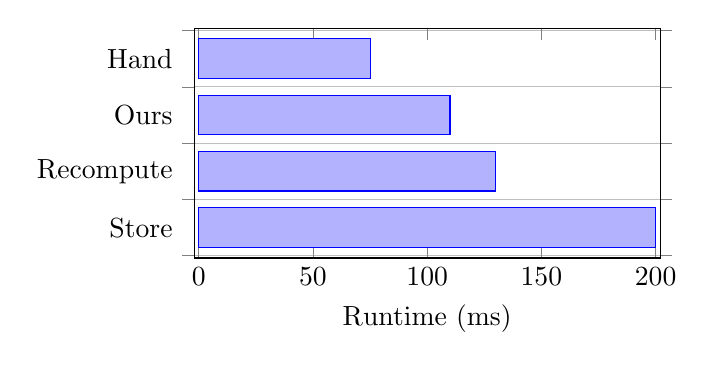
\begin{tikzpicture}
\begin{axis}[
  symbolic y coords={Store, Recompute, Ours, Hand, end},
	xlabel=Runtime (ms),
  xmin=0, xmax=200,
	enlargelimits=0.01,
	xbar interval=0.7,
  width=7.5cm, height=4.5cm,
	legend pos=north west,
]
\addplot coordinates {(200,Store) (130,Recompute) (110,Ours) (75,Hand) (0,end) };
\end{axis}
\end{tikzpicture}
\caption{Runtime for Quickhull; lower is faster.}
\label{fig:bench:quickhull}
\end{figure}

\subsection{Quickhull}
Quickhull is a divide-and-conquer spatial algorithm to find the smallest convex hull containing all points.
At its core is an operation called `filterMax', which takes a line and an array of points, and computes the maximum distance from the line, as well as all points that are above the line.
In our system this can be fused into a single loop, while shortcut-fusion systems do not support horizontal fusion.

We compare hand-fused against ours, as well as two @Data.Vector@ versions, which uses shortcut fusion.
The shortcut fusion system cannot fuse both operations into a single loop, and both operations require the distances between the line and each point.
This means a choice must be made: either compute the distances upfront and share them, or recompute the distances in each operation.
For our benchmarks we implemented both, and recomputing was significantly faster.
However, it is worth noting that we only benchmarked with two-dimensional points: at higher dimensions, the cost of recomputing distances may outweigh the cost of array allocation.

\autoref{fig:bench:quickhull} shows the runtimes for Quickhull over roughly 80MB of data, or five million points.
The hand-fused version is the fastest, while our version is slower, but still faster than the two vector versions.
The fact that our version is slower than the hand-fused version is surprising, as the generated GHC core is almost identical: the only difference is an extra continuation bound inside the loop, which acts as a sort of indirect jump in the recursive case.
It is possible that recent work on optimising continuations in GHC~\cite{downen2016sequent} will solve this.

\begin{figure}
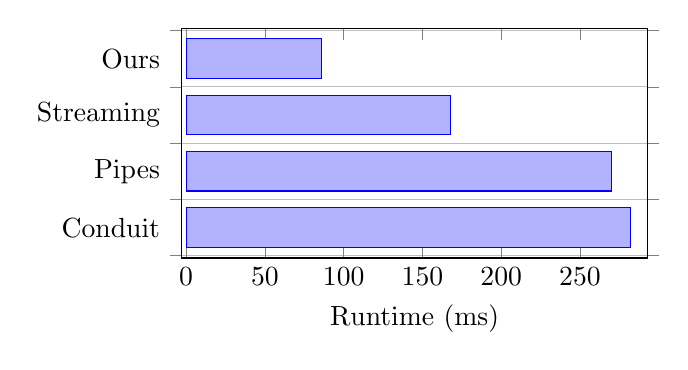
\begin{tikzpicture}
\begin{axis}[
  symbolic y coords={Conduit, Pipes, Streaming, Ours, end},
	xlabel=Runtime (ms),
  xmin=0, xmax=290,
	enlargelimits=0.01,
	xbar interval=0.7,
  width=7.5cm, height=4.5cm,
	legend pos=north west,
]
\addplot coordinates {(282,Conduit) (270,Pipes) (168,Streaming) (86,Ours) (0,end) };
\end{axis}
\end{tikzpicture}
\caption{Runtime for append2; lower is faster.}
\label{fig:bench:append}
\end{figure}

\subsection{Append files}
The first file-based benchmark consists of appending two files, while counting the number of lines.
We have benchmarked against three Haskell streaming libraries: Conduit, Pipes, and Streaming.
\autoref{fig:bench:append} shows the runtimes for appending 1.8MB of data.
The absolute performance here is poor because all are using line-buffered IO; in practice one would use chunked IO, but the overhead per chunk would remain.


\begin{figure}
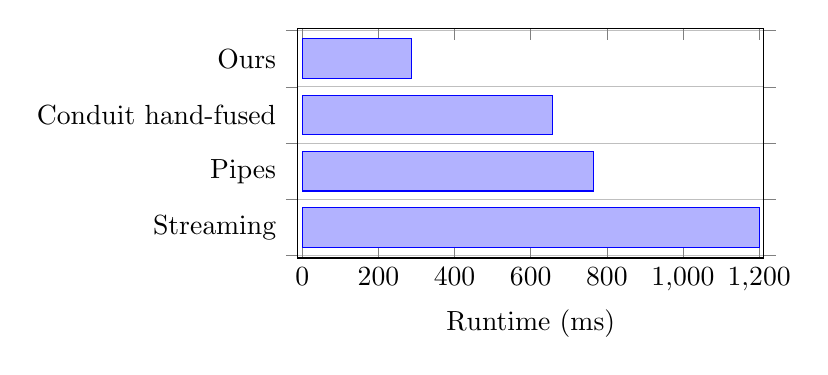
\begin{tikzpicture}
\begin{axis}[
  symbolic y coords={Streaming, Pipes, Conduit hand-fused, Ours, end},
	xlabel=Runtime (ms),
  xmin=0, xmax=1200,
	enlargelimits=0.01,
	xbar interval=0.7,
  width=7.5cm, height=4.5cm,
	legend pos=north west,
]
\addplot coordinates {(1200,Streaming) (764,Pipes) (658,Conduit hand-fused) (288,Ours) (0,end) };
\end{axis}
\end{tikzpicture}
\caption{Runtime for partition; lower is faster.}
\label{fig:bench:part}
\end{figure}

\subsection{Partition file}
The second file-based benchmark takes a single input file and partitions it into two files: one with even-length lines, and one with odd-length lines.
The number of lines in each output file is also counted.
The three streaming libraries are pull-based, and so do not support multiple outputs; the program must be written in a convoluted way or at least partially hand-fused.
Even with hand-fusion, the Pipes and Conduit programs are slower than ours, as well as losing any abstraction benefits from using a streaming library.
\autoref{fig:bench:part} shows the runtimes for partitioning a file into two.



%!TEX root = ../Main.tex

\section{Proofs}
\label{s:Proofs}

Our fusion system is formalized in Coq, and we have proved soundness of \ti{fusePair}: if the fused result process produces a particular sequence of values on its output channels then the two source processes may also produce that same sequence. The converse is not true, however: concurrent evaluation represents all possible interleavings, of which the fused process is only one.

% Note that the converse is not necessarily true: just because two processes can evaluate to a particular output does not mean the fused program will evaluate to that. This is because, as explained in~\S\ref{s:EvaluationOrder}, evaluation of a process network is non-deterministic, and fusion commits to a particular evaluation order.

\begin{code}
Theorem Soundness 
  (P1 : Program L1 C V1) (P2 : Program L2 C V2)
  (ss : Streams) (h : Heap) (l1 : L1) (l2 : L2)
  (is1 : InputStates) (is2 : InputStates) 
  :  EvalBs (fuse P1 P2) ss h (LX l1 l2 is1 is2)
  -> EvalOriginal Var1 P1 P2 is1 ss h l1
  /\ EvalOriginal Var2 P2 P1 is2 ss h l2.
\end{code}

@EvalBs@ evaluates the fused program, and @EvalOriginal@ ensures that the original program evaluates with that program's subset of the result heap. The Coq formalization has some small differences from the system in this paper. Instead of implementing non-deterministic evaluation we sequentially evaluate each source processes independently, and compare the output values to the ones produced by sequential evaluation of the fused result process. This is sufficient for our purposes because we are mainly interested in the value correctness of the fused program, rather than making a statement about the possible execution orders of the source processes when run concurrently.

% Care must be taken to remove stream values that the other process has pulled but this one has not yet.
%%% AR: Really would like to say something about this but no room to explain properly
% For shared inputs when one program has pulled, the other program must be evaluated with the other value removed from the end of the stream.

% Firstly, the Coq formalization uses a separate @update@ instruction to modify variables in the local heap, rather than attaching heap updates to the \Next~ label of every instruction. Performing this desugaring makes the low level lemmas easier to prove, but we find attaching the updates to each instruction makes for an easier exposition. Secondly, our formalization only implements sequential evaluation for a single process, rather than non-deterministic evaluation for whole process groups as per Figure~\ref{fig:Process:Eval:Feed}. Instead, we sequentially evaluate each source processes independently, and compare the output values to the ones produced by sequential evaluation of the fused result process. This is sufficient for our purposes because we are mainly interested in the value correctness of the fused program, rather than making a statement about the possible execution orders of the source processes when run concurrently.

% This causes the fusion definition to be slightly more complicated, as two output instructions must be emitted when performing a push or pull followed by an update. This is a fairly minor difference, and we have made this change in the paper version for ease of exposition.
% Ideally, a future version of the formalisation would include this change.
% Secondly, our formalisation does not implement the concurrent evaluation semantics for processes, only sequential evaluation for a single process. Instead we sequentially evaluate both processes with the same input values and outputs. Despite these differences, the Coq formalisation gives us sufficient confidence in the correctness of the version presented here.


%!TEX root = ../Main.tex
\eject
\section{Related work}

This work aims to address the limitations of current combinator-based array fusion systems. As stated in the introduction, neither pull-based or push-based fusion is sufficient. Some combinators are inherently push-based, particularly those with multiple outputs such as @unzip@; while others are inherently pull-based, such as @zip@.

% Short cut fusion is an attractive idea, as it allows fusion systems to be specified by a single rewrite rule. Thus, short cut fusion is inherently biased towards pull fusion.

However, short cut fusion \cite{gill1993short} relies on inlining which, like pull-based streams, only occurs when there is a single consumer. Push-based short cut fusion systems \emph{do} exist, notably the original foldr/build formulation, but support neither @zip@ nor @unzip@ \cite{svenningsson2002shortcut,lippmeier2013data}.

Recent work on stream fusion \cite{kiselyov2016stream} uses staged computation in a push-based system to ensure all combinators are inlined. When streams are used multiple times this causes excessive inlining, which duplicates work. This can change the semantics for effectful streams.

% For effectful inputs such as reading from the network, duplicating work changes the semantics.
% I could write more about this eg only supporting a single output, but the other points probably apply to push streams in general

Data flow fusion~\cite{lippmeier2013data} is neither pull-based nor push-based, and supports arbitrary splits and joins. It supports only a fixed set of standard combinators such as @map@, @filter@ and @fold@, and converts each stream to a series with explicit rate types, similar to the clock types of Lucid Synchrone \cite{benveniste2003synchronous}.
% These rate types ensure that well-typed programs can be fused without introducing unbounded buffers.
% This allows unfusable programs to be caught at compile time.
% However, it only supports a limited set of combinators, and adding more is non-trivial.

One way to address the difference between pull and push streams is to explicitly support both \cite{bernardy2015duality, lippmeier2016polarized}. Here, pull streams have the type @Source@ and represent a source, always ready to be pulled, while push streams have the type @Sink@ and represent a sink, always ready to accept data. The addition of push streams allows more programs to be fused than pull-only systems, but the computation must be manually split into sources and sinks.

% This system requires the streaming computation to be manually split into sources and sinks.
% Both systems rely on stream bindings being used linearly to ensure correctness.
% Operations over sources are expressed fairly naturally compared to streams, for example the @zip@ combinator has the type @Source a -> Source b -> Source (a,b)@.
% Sinks are co-variant, and operations must be performed somewhat backwards, so that the @unzip@ combinator takes the two output sinks to push into and returns a new sink that pushes into these.
% It has the type @Sink a -> Sink b -> Sink (a,b)@.
% and be joined together by a loop that `drains' values from the source and pushes them into the sink.

The duality between pull and push arrays has also been explored in Obsidian \cite{claessen2012expressive, svensson2014defunctionalizing}. Here the distinction is made for the purpose of code generation for GPUs rather than fusion, as operations such as appending pull arrays require conditionals inside the loop, whereas using push arrays moves these conditionals outside the loop.

Meta-repa \cite{ankner2013edsl} supports both array types in a similar way, using Template Haskell for code generation. It supports fusion on both array types. When arrays are used multiple times, they must be explicitly reified with a `force' operation to avoid duplication.


Streaming IO libraries have blossomed in the Haskell ecosystem, generally based on Iteratees \cite{kiselyov2012iteratees}. Libraries such as @conduit@ \cite{hackage:conduit}, @enumerator@ \cite{hackage:enumerator}, @machines@ \cite{hackage:machines} and @pipes@ \cite{hackage:pipes} are all designed to write stream computations with bounded buffers, but do not guarantee fusion.

% However, these libraries do not guarantee fusion guarantees, and as such programs tend to be written over chunks of data to make up for the communication overhead.

% For the most part they support only straight-line computations, with only limited forms of branching.

Like our own Machine Fusion,  Filter Fusion~\cite{proebsting1996filter} also statically interleaves the code of producer and consumer processes. Each process must have a single input and output channel, so common operators like @zip@, @unzip@, @append@, @partition@ and so on are not supported. Given an adjacent producer and consumer pair, Filter Fusion alternately assigns control to the code of each. When the consumer needs input, control is passed to the producer, and when the producer produces its value control is passed back to the consumer. This simple scheduling algorithm works only for straight line pipelines of processes. Machine fusion provides a finer grained interleaving of code, which is nessesary to support branching dataflows that contain both splits and joins.

%Filter Fusion~\cite{proebsting1996filter} uses a similar algorithm, but only supports processes with at most one input and one output channel.
% This means combinators such as @zip@, @unzip@, @append@, and @partition@ cannot be expressed.
%Also, the process network must be a straight line, with no splits or joins.
%Here a consumer and a producer are fused by alternating between the two; when the consumer needs input, control is passed to the producer, and when the producer has output, control is passed to the consumer.
%This is sufficient when only one channel is shared, but when multiple channels are shared finer-grained coordination is required.

% This is sufficient for producer-consumer fusion, but two consumers pulling from the same input channel need not follow the same alternation.
% This is sufficient when only one , but when multiple channels are shared between two processes, as may be the case in an intermediate fused result of a larger program, it is not obvious whether simply alternating the two processes is correct.

% The synchronised product of two processes allows either process to take independent or local steps at any time, but shared actions, such as when both processes communicate on the same channel, must be taken in both processes at the same time.
% When two processes share multiple channels, synchronised product will fail unless both processes read the channels in exactly the same order.
% In our system the use of stream buffer variables allows some leeway in when processes must take shared steps.

% This is a much simpler fusion method than ours, but is also much stricter.

% They do not have to take shared steps at the same time, but if one process lags behind the other, it must catch up before the other one gets too far ahead.

Synchronous languages such as LUSTRE~\cite{halbwachs1991synchronous}, Lucy-n~\cite{mandel2010lucy} and SIGNAL~\cite{le2003polychrony} all use some form of clock calculus and causality analysis to ensure that programs can be statically scheduled with bounded buffers~\cite{caspi1996:kahn}. These languages describe \emph{passive} processes where values are fed in to streams from outside environments, such as data coming from sensors. In contrast, our processes are \emph{active} and have control over when data is pulled from the source streams, which is nessesary for multiple input combinators such as @merge@ and  @append@.
Synchronous dataflow languages reject operators with value dependent control flow such as @merge@, while general dataflow languages fall back on less performant dynamic scheduling \cite{bouakaz2013real}.


% In this case, the passive process has no control over the rate of input coming in, and if they support multiple input streams, they must accept values from them in any order.


% Note that in the synchronous language literature, it is common to refer to a different merge operation, also known as @default@, which computes a stream that is defined whenever either input is defined.

Synchronous dataflow (SDF; not to be confused with synchronous languages above) is a dataflow graph model of computation where each node has constant, statically known input and output rates. StreamIt~\cite{thies2002streamit} uses synchronous dataflow for scheduling when possible, otherwise falling back to dynamic scheduling~\cite{soule2013dynamic}. Boolean dataflow and integer dataflow~\cite{buck1993scheduling,buck1994static} extend SDF with boolean and integer valued control ports, but only support limited control flow.


% SDF is simple enough for static scheduling to be decidable, but this comes at a cost of expressivity.

% Finite state machine-based scenario aware dataflow (FSM-SADF)~\cite{stuijk2011scenario,van2015scenario} is quite expressive compared to boolean and integer dataflow, while still ensuring static scheduling. A finite state machine is constructed, where each node of the FSM denotes its own SDF graph. The FSM transitions from one dataflow graph to another based on control outputs of the currently executing dataflow graph. For example, a filter is represented with two nodes in the FSM. The initial state executes the predicate, and the value of the predicate is used to determine which transition the FSM takes: either the predicate is false and the FSM stays where it is, or the predicate is true and moves to the next state. The next state emits the value, and returns to the start. This appears to be able to express value-dependent operations such as merge, but lacks the composability and familiarity of combinators.

% StreamIt:
% Only allows limited splits and joins: round robin and duplication for splits, round robin and combination for joins.
% Does not support fully general graphs - instead using combinators to introduce a (split/join) and a combinator for a feedback loop.
%
% Parameterized dataflow (PDF),  \cite{bhattacharya2001parameterized}
% Schedulable parametric dataflow (SPDF),  \cite{fradet2012spdf}

% Recent work on stream fusion by \citet{kiselyov2016stream} uses staged computation to ensure all combinators are inlined, but for splits this causes excessive inlining which duplicates work, due to values of the source arrays being read multiple times.


% %!TEX root = ../Main.tex

% -----------------------------------------------------------------------------
\section{Future work}
\label{s:FutureWork}

%%% AR: Can we fit a few sentences here just to conclude, say we've described a fusion algorithm, with promising future work too

\subsection{Case analysis}
\label{s:FullyAbstractCase}

The fusion algorithm treats all @case@ conditions as fully abstract by exploring all possible combinations for both processes.
This can cause issues for processes that dynamically require only a bounded buffer, but the fusion algorithm statically tries every combination and wrongly asserts that unbounded buffering is required.

For example, if two processes have the same case condition (@x > 0@), the fusion algorithm generates all four possibilities, including contradictory ones where one process is true and the other is false.
If any require an unbounded buffer, the fusion algorithm fails.

One solution may be to cull contradictory states so that if it is statically known that a state is unreachable, it does not matter if it requires unbounded buffers.
It may be possible to achieve this with relatively little change to the fusion algorithm itself, by having it emit a failure instruction rather than failing to produce a process.
A separate postprocessing step could then remove statically unreachable process states.
After postprocessing, if any failure instructions are reachable, fusion fails as before.




% -----------------------------------------------------------------------------
% \subsection{Non-determinism and fusion order}
% \label{s:FusionOrder}
% The main fusion algorithm here works on pairs of processes.
% When there are more than two processes, there are multiple orders in which the pairs of processes can be fused. The order in which pairs of processes are fused does not affect the output values, but it does affect the access pattern: the order in which outputs are produced and inputs read. Importantly, the access pattern also affects whether fusion succeeds or fails to produce a process. In other words, while evaluating multiple processes is non-deterministic, the act of fusing two processes \emph{commits} to a particular deterministic interleaving of the two processes. The simplest example of this has two input streams, a function applied to both, then zipped together. 
% \begin{code}
% zipMap as bs =
%   let as' = map (+1) as
%       bs' = map (+1) bs
%       abs = zip as' bs'
%   in  abs
% \end{code}
% There are three combinators here, so after converting each combinator to its process there are three orders we can fuse. The two main options are to fuse the two maps together and then add the zip, or to fuse the zip with one of the maps, then add the other map. If we start by fusing the zip with one of its maps, the zip ensures that its inputs are produced in lock-step pairs, and then adding the other map will succeed. However if we try to fuse the two maps together, there are many possible interleavings: the fused program could read all of @as'@ first; it could read all of @bs'@ first; it read the two in lock-step pairs; or any combination of these. When the zip is added, fusion will fail if the wrong interleaving was chosen.

% The example above can be solved by fusing connected processes first, but it is possible to construct a connected process that still relies on the order of fusion.
% 
% \begin{code}
% zipApps as bs cs =
%   let as' = as ++ bs
%       bs' = as ++ cs
%       abs = zip as' bs'
%   in  abs
% \end{code}

% \subsection{Non-determinism and fusion order}
% \label{s:Future:FusionOrder}
% Our current solution to this is to try all permutations of fusing processes and use the first one that succeeds. A more principled solution may be to allow non-determinism in a single process by adding a non-deterministic choice instruction. Then when fusing two processes together, if both processes are pulling from unrelated streams, the result would be a non-deterministic choice between pulling from the first process and executing the first, or pulling from the second process and executing the second. In this way we could defer committing to a particular evaluation order until the required order is known. This may produce larger intermediate programs, but the same deterministic program could be extracted at the end.



\bibliography{Main}

%%% "Extended paper"
% \appendix
% %!TEX root = ../Appendix.tex
\clearpage{}

\section{Finite streams}
\label{s:FiniteDetails}

This appendix briefly describes the finite streams extension, showing the changes to instructions and the fusion algorithm.
The finite evaluation rules are not shown, as the changes follow the same structure as the changes to the fusion algorithm.


Figure~\ref{fig:Finite:Instr} shows the grammar for instructions and the static input state. The first group of instructions containing @push@, @drop@, @case@ and @jump@ are unchanged.

The @pull@ instruction is modified to have two output labels, similar to @case@. The first, the success branch, is used when the input stream is still open and pulling succeeds, in which case the variable is set to the pulled value as before. The second output label, the closed branch, is used when the input stream has been closed, and the variable is not written to. This new @pull@ is analogous to a @pull@ followed by a @case@ in the infinite stream version.

The @close@ instruction is used by a pushing process to close or end an output stream. Any subsequent pulls from this channel in other processes will take the closed branch. After an output channel is closed, it cannot be pushed to and remains closed forever.

Finally, the @exit@ instruction is used once a process is finished with all its streams, and has nothing left to do. All output streams must be closed before the process finishes. This instruction has no output labels, as there is nothing further to execute.

Also in Figure~\ref{fig:Finite:Instr}, the static input state used for fusion ($\InputStateF$) must now track closed streams. The new constructor $@closed@_F$ denotes that the stream is closed, while the rest is unchanged.

For the fusion algorithm, the top-level function $\ti{fusePair}$ remains unchanged. The functions $\ti{outlabels}$ and $\ti{swaplabels}$ are not shown as they are easily modified by adding cases for the new instructions.

Figure~\ref{fig:Finite:tryStepPair} shows the modified $\ti{tryStepPair}$ function. This function uses the same heuristics to decide which process to execute when both can progress, but now that the processes can finish with @exit@, we must take care to only finish the fused process once \emph{both} source processes are finished. The (DeferExit1) and (DeferExit2) clauses achieve this by forcing the other process to run if one is an @exit@. Once both processes are finished, both new clauses will fail while (Run1) succeeds, using the @exit@ from the first process. Another way to think of this is that if either process has work to do, the fused process still has work to do.

Figure~\ref{fig:Finite:tryStep} shows the modified $\ti{tryStep}$ function.
The clauses for the unchanged instructions @push@, @drop@, @case@ and @jump@ remain unchanged; these are reordered to the top of the function.

The @pull@ clauses use $l'_o$ for the open output label, and $l'_c$ for the closed label.
Clause (LocalPull) now uses two output labels, and leaves the other process as-is.

Clause (SharedPull) applies when the channel state is @pending@, meaning there is already a value available. This means that the channel is not yet closed, and the success branch can be taken.

Clause (SharedPullInject) applies when both processes need to pull from a shared input. As before, we execute a real @pull@, this time with two branches. In the success branch, the input states are set to @pending@ as before. In the closed branch, the input states are set to @closed@ so the next and subsequent pulls take the closed branch.

Clause (SharedPullClosed) applies when the channel state is @closed@, which means either the other process has pulled and discovered that the channel is closed, or in case of connected input, the other process has closed the channel. Either way we simply jump, taking the closed branch of the @pull@.

Clause (LocalClose) applies when closing a local output.

Clause (SharedClose) applies when closing a connected output. As with (SharedPush), the other input state for the other process must be empty and ready to pull from the channel. The input state for the other process is then set to @closed@, forcing its next pull to take the closed branch.

Finally, clause (LocalExit) allows the process to finish. However, recall that the $\ti{tryStepPair}$ function has been modified to only @exit@ when both processes are ready to finish.


\begin{figure}
\begin{tabbing}
MMMMMM \TABDEF @MMMMM@  \TABSKIP $\Chan$ \TABSKIP $\Chan$ \TABSKIP $\Next$ \TABSKIP \kill
\Instr
    \> ::=\> @push@  \> \Chan  \> \Exp  \> \Next \\
    \TABALT  @drop@  \> \Chan  \>       \> \Next \\
    \TABALT  @case@  \> \Exp   \> \Next \> \Next \\
    \TABALT  @jump@  \>        \>       \> \Next \\
    \\
    \TABALT  @pull@  \> \Chan  \> \Var  \> \Next \> \Next \\
    \TABALT  @close@ \> \Chan  \>       \> \Next \\
    \TABALT  @exit@ 
\\
\\
$\InputStateF$ \> ::=  \> ~~~ $@none@_F ~|~ @pending@_F ~|~ @have@_F ~|~ @closed@_F$
\end{tabbing}
\caption{Finite instructions}
\label{fig:Finite:Instr}
\end{figure}


% -----------------------------------------------------------------------------
\begin{figure}
\begin{tabbing}
\ti{tryStepPair}\=$~\to~$\=M\kill

$\ti{tryStepPair} ~:~ \ChanTypeMap$ \\
\> $\to$ \> $\LabelF \to \Instr \to \LabelF \to \Instr$ \\
\> $\to$ \> $\Maybe~\Instr$ \\

M \= $~|~(@pull@~\_~\_~\_ \gets i_p')~$ \= $\to$ \= $\Just (\ti{swaplabels}~i_q')~$ \= M \=\kill
$\ti{tryStepPair} ~\cs~l_p~i_p~l_q~i_q~=$ \\
\> $@match@~ (\ti{tryStep}~\cs~l_p~i_p~l_q,~\ti{tryStep}~\cs~l_q~i_q~l_p) ~@with@$ \\
\> $(\Just i_p',~\Just i_q')$ \\

\> @ @$|~@exit@ \gets i_q'$ \> $\to$ \> $\Just i_p'$
\> \note{DeferExit1} \\[0.5ex]

\> @ @$|~@exit@ \gets i_p'$ \> $\to$ \> $\Just (\ti{swaplabels}~i_q')$
\> \note{DeferExit2} \\[0.5ex]

\> @ @$|~@jump@~\_ \gets i_p'$ \> $\to$ \> $\Just i_p'$
\> \note{PreferJump1} \\[0.5ex]

\> @ @$|~@jump@~\_ \gets i_q'$ \> $\to$ \> $\Just (\ti{swaplabels}~i_q')$
\> \note{PreferJump2} \\[0.5ex]

\> @ @$|~@pull@~\_~\_~\_ \gets i_q'$ \> $\to$ \> $\Just i_p'$
\> \note{DeferPull1} \\[0.5ex]

\> @ @$|~@pull@~\_~\_~\_ \gets i_p'$ \> $\to$ \> $\Just (\ti{swaplabels}~i_q')$
\> \note{DeferPull2} \\[0.5ex]

\> $(\Just i_p',~\_)$ \> $\to$ \> $\Just i_p'$
\> \note{Run1} \\[0.5ex]

\> $(\_, ~\Just i_q')$ \> $\to$ \> $\Just (\ti{swaplabels}~i_q')$
\> \note{Run2} \\[0.5ex]

\> $(\Nothing, ~\Nothing)$ \> $\to$ \> $\Nothing$
\> \note{Deadlock}
\end{tabbing}
\caption{Fusion step coordination for a pair of processes.}
\label{fig:Finite:tryStepPair}
\end{figure}


% -----------------------------------------------------------------------------
\begin{figure*}
\begin{tabbing}
M \= M \= MMMMMMMMMMMMMMMMMMMMMM \= MMMMMMMMMMMMMMMMMMMMMMMMMMMMMM \= \kill
$\ti{tryStep} ~:~ \ChanTypeMap \to \LabelF \to \Instr \to \LabelF \to \Maybe~\Instr$ \\
$\ti{tryStep} ~\cs~(l_p,s_p)~i_p~(l_q,s_q)~=~@match@~i_p~@with@$ \\

\> $@jump@~(l',u')$ 
\> \> $\to~\Just (@jump@~
      \nextStep
        {l'}{s_p}
        {l_q}{s_q}
        {u'})
      $ 
\> \note{LocalJump}
\\[1ex]

\> $@case@~e~(l'_t,u'_t)~(l'_f,u'_f)$
\> \> $\to~\Just (@case@~e~
      \nextStep
        {l'_t}{s_p}
        {l_q}{s_q}
        {u'_t}
      ~
      \nextStep
        {l'_f}{s_p}
        {l_q}{s_q}
        {u'_f})
      $ 
\> \note{LocalCase}
\\[1ex]

\> $@push@~c~e~(l',u')$ \\
\> \> $~|~\cs[c]=@out1@$ 
\\
\> \> $\to~\Just (@push@~c~e~
      \nextStep
        {l'}
          {s_p}
        {l_q}
          {s_q}
        {u'})
      $ 
\> \> \note{LocalPush}\\

\> \> $~|~\cs[c]=@in1out1@ ~\wedge~ s_q[c]=@none@_F$ 
\\
\> \> $\to~\Just (@push@~c~e~
      \nextStep
        {l'}
          {s_p}
        {l_q}
          {\HeapUpdateOne{c}{@pending@_F}{s_q}}
        {\HeapUpdateOne{@chan@~c}{e}{u'}})
      $
\> \> \note{SharedPush}
\\[1ex]

\> $@drop@~c~(l',u')$ \\
\> \> $~|~\cs[c]=@in1@$
\> \hspace{2em} $\to~\Just (@drop@~c~
      \nextStep
        {l'}
          {s_p}
        {l_q}
          {s_q}
        {u'})
      $
\> \note{LocalDrop} \\

\> \> $~|~\cs[c]=@in1out1@$
\> \hspace{2em} $\to~\Just (@jump@~
      \nextStep
        {l'}
          {\HeapUpdateOne{c}{@none@_F}{s_p}}
        {l_q}
          {s_q}
        {u'})
      $
\> \note{ConnectedDrop}\\

\> \> $~|~\cs[c]=@in2@ ~\wedge~ (s_q[c]=@have@_F \vee s_q[c]=@pending@_F)$ 
\> \hspace{2em} $\to~\Just (@jump@~
      \nextStep
        {l'}
          {\HeapUpdateOne{c}{@none@_F}{s_p}}
        {l_q}
          {s_q}
        {u'})
      $
\> \note{SharedDropOne}\\



\> \> $~|~\cs[c]=@in2@ ~\wedge~ s_q[c]=@none@_F$
\> \hspace{2em} $\to~\Just (@drop@~c~
      \nextStep
        {l'}
          {\HeapUpdateOne{c}{@none@_F}{s_p}}
        {l_q}
          {s_q}
        {u'})
      $
\> \note{SharedDropBoth}
\\[1ex]

\\



\> $@pull@~c~x~(l'_o,u'_o)~(l'_c,u'_c)$ \\
\> \> $~|~\cs[c]=@in1@$ 
\\
\> \> $\to~\Just (@pull@~c~x~
      \nextStep
        {l'_o}{s_p}
        {l_q}{s_q}
        {u'_o}
      ~
      \nextStep
        {l'_c}{s_p}
        {l_q}{s_q}
        {u'_c})
    $ 
\> \> \note{LocalPull}
\\[1ex]

\> \> $~|~(\cs[c]=@in2@ \vee \cs[c]=@in1out1@) ~\wedge~ s_p[c]=@pending@_F$ \\
\> \> $\to~\Just (@jump@~
      \nextStep
        {l'_o}
          {\HeapUpdateOne{c}{@have@_F}{s_p}}
        {l_q}
          {s_q}
        {\HeapUpdateOne{x}{@chan@~c}{u'_o}})
        $ 
\> \> \note{SharedPull} 
\\[1ex]

\> \> $~|~\cs[c]=@in2@ ~\wedge~ s_p[c]=@none@_F ~\wedge~ s_q[c]=@none@_F$ \\
\> \> $\to~\Just (@pull@~c~(@chan@~c)~
      \nextStep
        {l_p}
          {\HeapUpdateOne{c}{@pending@_F}{s_p}}
        {l_q}
          {\HeapUpdateOne{c}{@pending@_F}{s_q}}
        {[]}$
      \\
\> \> @                     @
      $\nextStep
        {l_p}
          {\HeapUpdateOne{c}{@closed@_F}{s_p}}
        {l_q}
          {\HeapUpdateOne{c}{@closed@_F}{s_q}}
        {[]})
  $
\> \> \note{SharedPullInject}
\\[1ex]

\> \> $~|~(\cs[c]=@in2@ \vee \cs[c]=@in1out1@) ~\wedge~ s_p[c]=@closed@_F$ \\
\> \> $\to~\Just (@jump@~
      \nextStep
        {l'_c}{s_p}
        {l_q}{s_q}
        {u'_c})
  $
\> \> \note{SharedPullClosed}
\\[1ex]

\> $@close@~c~(l',u')$ \\
\> \> $~|~\cs[c]=@out1@$ 
\> $\to~\Just (@close@~c~
      \nextStep
        {l'}{s_p}
        {l_q}{s_q}
        {u'})
    $ 
\> \note{LocalClose}
\\

\> \> $~|~\cs[c]=@in1out1@ ~\wedge~ s_q[c]=@none@_F$ 
\> $\to~\Just (@close@~c~
      \nextStep
        {l'}{s_p}
        {l_q}{\HeapUpdateOne{c}{@closed@_F}{s_q}}
        {u'})
    $ 
\> \note{SharedClose}
\\[1ex]

\> $@exit@$
\> 
\> $\to~\Just @exit@$
\> \note{LocalExit}
\\[1ex]


% \> @otherwise@ \>
\> $\_$ \> $~|~ @otherwise@ $
\> $\to ~ \Nothing$
\> \note{Blocked}


\end{tabbing}

\caption{Fusion step for a single process of the pair.} 

\label{fig:Finite:tryStep}
\end{figure*}

\clearpage{}
% %!TEX root = ../Appendix.tex

\clearpage{}
\section{Result Size}
\label{s:ResultSize}

As with any fusion system, we must be careful that the size of the result code does not become too large when more and more processes are fused together. 

\subsection{Fusing Pipelines of Processes}
The following figure shows the maximum number of output states in the result when a particular number of processes are fused together in a pipelined-manner.

\smallskip
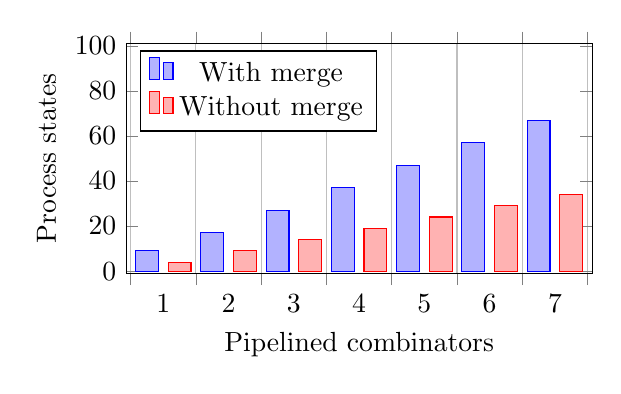
\begin{tikzpicture}
\begin{axis}[
% Hide the label on the second graph
        ylabel=Process states,
        xlabel=Pipelined combinators,
  ymin=0, ymax=100,
        enlargelimits=0.01,
        ybar interval=0.7,
  width=7.5cm, height=4.5cm,
        legend pos=north west,
]
\addplot coordinates {(1,9) (2,17) (3,27) (4,37) (5,47) (6,57) (7,67)   (8,1) };
\addplot coordinates {(1,4) (2,9) (3,14) (4,19) (5,24) (6,29) (7,34)    (8,1) };
\legend{With merge, Without merge};
\end{axis}
\end{tikzpicture}


To produce the above graph we programmatically generated dataflow networks for \emph{all possible} pipelined combinations of the @map@, @filter@, @scan@, @group@ and @merge@ combinators, and tried all possible fusion orders consiting of adjacent pairs of processes. The @merge@ combinator itself has two inputs, so only works at the very start of the pipeline --- we present result for pipelines with and without a @merge@ at the start. 

\subsection{Fusing Parallel Processes}
The following figure shows the number of states in the result when the various combinations of combinators are fused in parallel, for example, we might have a @map@ and a @filter@ processing the same input stream. In both cases the number of states in the result process grows linearly with the number of processes. In all combinations, with up to 7 processes there are less than 100 states in the result process.

\smallskip
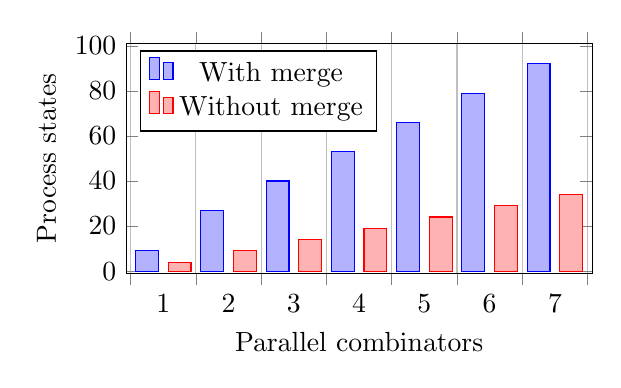
\begin{tikzpicture}
\begin{axis}[
        ylabel=Process states,
        xlabel=Parallel combinators,
  ymin=0, ymax=100,
        enlargelimits=0.01,
        ybar interval=0.7,
  width=7.5cm, height=4.5cm,
        legend pos=north west,
]
\addplot coordinates {(1,9) (2,27) (3,40) (4,53) (5,66) (6,79) (7,92)
  % Last bar doesn't show for some reason, so need to add a dummy value for the next one
    (8,1) };

\addplot coordinates {(1,4) (2,9) (3,14) (4,19) (5,24) (6,29) (7,34)    (8,1) };

\legend{With merge, Without merge};
\end{axis}
\end{tikzpicture}

The size of the result process is roughly what one would get when inlining the definitions of each of the original source processes. This is common with other systems based on inlining and/or template meta-programming, and is not prohibitive.


\eject{}
% -----------------------------------------------------------------------------
\subsection{Fusing Merges}

On the other hand, the following figure shows the results for a pathological case where the size of the output program is exponential in the number of input processes. The source dataflow networks consists of N merge processes, N+1 input streams, and a single output stream. The output of each merge process is the input of the next, forming a chain of merges. In source notation the network for N = 3 is @sOut = merge sIn1 (merge sIn2 (merge sIn3 sIn4))@.

\medskip
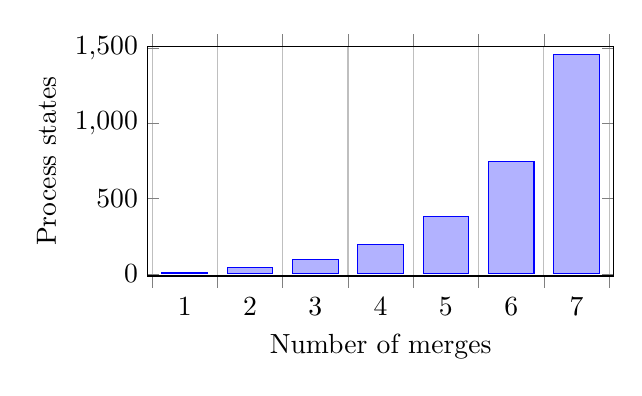
\begin{tikzpicture}
\begin{axis}[
        ylabel=Process states,
        xlabel=Number of merges,
%  ymode=log,
  ymin=0, ymax=1500,
        enlargelimits=0.01,
        ybar interval=0.7,
  width=7.5cm, height=4.5cm,
        legend pos=north west,
]
% These are the values for splitting.
% They are smaller than the 'chaining', but look much nicer on the linear graph.
\addplot coordinates {(1,9) (2,42) (3,97) (4,196) (5,383) (6,746) (7,1461)
  % (8,2880)
  (8,1)
  };

% These are the values for chaining
% \addplot coordinates {(1,4) (2,48) (3,194) (4,760) (5,2814) (6,10064) (7,1) };

\end{axis}
\end{tikzpicture}


When fusing two processes the fusion algorithm essentially compares every state in the first process with every state in the second, computing a cross product. During the fusion transform, as states in the result process are generated they are added to a finite map --- the @instrs@ field of the process definition. The use of the finite map ensures that identical states are always combined, but genuinely different states always make it into the result. 
In the worst case, fusion of two processes produces O($n*m$) different states, where $n$ and $m$ are the number of states in each. If we assume the two processes have about the same number of states then this is O($n^2$). Fusing the next process into this result yields O($n^3$), so overall the worst case number of states in the result will be O($n^k$), where $k$ is the number of processes fused. 

In the particular case of @merge@, the implementation has two occurrences of the @push@ instruction. During fusion, the states for the consuming process are inlined at each occurrence of @push@. These states are legitimately different because at each occurence of @push@ the input channels of the merge process are in different channel states, and these channel states are included in the overall process state.


% \clearpage{}
% %!TEX root = ../Appendix.tex
\clearpage{}

\section{Combinators}
\label{s:Combinators}
Here we show the definitions of some combinators. We start with simple combinators supported by most streaming systems, and progress to more interesting combinators. Some standard combinators such as @fold@, @take@ and @append@ are missing due to the infinite nature of our streams, but could be implemented with the finite stream extension. The fact that segmented versions of these combinators can be implemented is compelling evidence of this.

Many of these combinators take a ``default'' argument, which is used to initialise the heap, but the stored value is never actually read. Ideally these could be left unspecified, or the heap left uninitialised in cases where it is never read.

\subsection{Map}
The map combinator applies a function to every element of the stream. This is some more text.

\begin{alltt}
map 
 =  \(\lambda\) (f : \(\alpha \to \beta\)) (default : \(\alpha\))
      (sIn: Stream \(\alpha\)) (sOut: Stream \(\beta\)). 
    \(\nu\) (a: \(\alpha\)) (L0..L2: Label).
\end{alltt}
\begin{code}
    process
    { ins:    { sIn }
    , outs:   { sOut }
    , heap:   { a = default }
    , label:  L0
    , instrs: { L0 = pull sIn     a  L1 []
              , L1 = push sOut (f a) L2 []
              , L2 = drop sIn        L0 [] } }
\end{code}


% -----------------------------------------------------------------------------
\subsection{Filter}
Filter returns a new stream containing only the elements that satisfy some predicate.
\begin{alltt}
filter 
 =  \(\lambda\) (f : \(\alpha \to\) Bool) (default : \(\alpha\))
      (sIn: Stream \(\alpha\)) (sOut: Stream \(\alpha\)). 
    \(\nu\) (a: \(\alpha\)) (L0..L3: Label).
\end{alltt}
\begin{code}
    process
    { ins:    { sIn }
    , outs:   { sOut }
    , heap:   { a = default }
    , label:  L0
    , instrs: { L0 = pull sIn  a     L1 []
              , L1 = case   (f a)    L2 []  L3 []
              , L2 = push sOut a     L3 []
              , L3 = drop sIn        L0 [] } }
\end{code}


\vspace{12em}
% -----------------------------------------------------------------------------
\subsection{Partition}
Partition is similar to filter, but has two output streams: those that satisfy the predicate, and those that do not. Partition is an inherently push-based operation, and cannot be supported by pull streams without buffering.
\begin{alltt}
partition 
 =  \(\lambda\) (f : \(\alpha \to\) Bool) (default : \(\alpha\))
      (sIn:   Stream \(\alpha\))
      (sOut1: Stream \(\alpha\)) (sOut2: Stream \(\alpha\)). 
    \(\nu\) (a: \(\alpha\)) (L0..L4: Label).
\end{alltt}
\begin{code}
    process
    { ins:    { sIn }
    , outs:   { sOut1, sOut2 }
    , heap:   { a = default }
    , label:  L0
    , instrs: { L0 = pull sIn   a    L1 []
              , L1 = case    (f a)   L2 []  L3 []
              , L2 = push sOut1 a    L4 []
              , L3 = push sOut2 a    L4 []
              , L4 = drop sIn        L0 [] } }
\end{code}


% -----------------------------------------------------------------------------
\subsection{Zip}
Zip, or zip-with, pairwise combines two input streams.
Zipping is an inherently pull-based operation.

\begin{alltt}
zipWith 
 =  \(\lambda\) (f : \(\alpha \to \beta \to \gamma\)) (default1 : \(\alpha\)) (default2 : \(\beta\))
      (sIn1: Stream \(\alpha\)) (sIn2: Stream \(\beta\))
      (sOut: Stream \(\gamma\)). 
    \(\nu\) (a: \(\alpha\)) (b : \(\beta\)) (L0..L4: Label).
\end{alltt}
\begin{code}
    process
    { ins:    { sIn1, sIn2 }
    , outs:   { sOut }
    , heap:   { a = default1, b = default2 }
    , label:  L0
    , instrs: { L0 = pull sIn1 a       L1 []
              , L1 = pull sIn2 b       L2 []
              , L2 = push sOut (f a b) L3 []
              , L3 = drop sIn1         L4 []
              , L4 = drop sIn2         L0 [] } }
\end{code}


% -----------------------------------------------------------------------------
\subsection{Scan}
Scan is similar to a fold, but instead of returning a single value at the end, it returns an intermediate value for each element of the stream.

\begin{alltt}
scan 
 =  \(\lambda\) (k : \(\alpha \to \beta \to \beta\)) (z : \(\beta\)) (default : \(\alpha\))
      (sIn: Stream \(\alpha\)) (sOut: Stream \(\beta\)).
    \(\nu\) (a: \(\alpha\)) (s : \(\beta\)) (L0..L2: Label).
\end{alltt}
\begin{code}
    process
    { ins:    { sIn  }
    , outs:   { sOut }
    , heap:   { a = default, s = z }
    , label:  L0
    , instrs: { L0 = pull sIn  a   L1 []
              , L1 = push sOut s   L2 [ s = f a s ]
              , L2 = drop sIn      L0 [] } }
\end{code}


% -----------------------------------------------------------------------------
\subsection{Segmented Fold}
Segmented fold performs a fold over each nested stream, using a segmented representation.
Here we are representing nested streams using one stream for the lengths of each substream, and another stream containing the values.
The output stream has the same rate as the lengths stream.
It reads a count (@c@) from the lengths stream, setting the fold state to zero (@z@).
Then it reads count times from the values stream, updating the fold state.
Afterwards, it pushes the final fold state, and continues to read a new count.

\begin{alltt}
folds 
 =  \(\lambda\) (k : \(\alpha \to \beta \to \beta\)) (z : \(\beta\)) (default : \(\alpha\))
      (sLens: Stream Nat) (sVals: Stream \(\alpha\))
      (sOut:  Stream \(\beta\)).
    \(\nu\) (c : Nat) (a: \(\alpha\)) (s : \(\beta\)) (L0..L5: Label).
\end{alltt}
\begin{code}
    process
    { ins:    { sLens, sVals }
    , outs:   { sOut }
    , heap:   { c = 0, a = default, s = z }
    , label:  L0
    , instrs: { L0 = pull sLens c   L1 [ s = z ]
              , L1 = case (c > 0)   L2 []  L4 []
              , L2 = pull sVals a   L3 []
              , L3 = drop sVals     L1 [ c = c - 1
                                       , s = k s a ]
              , L4 = push sOut  s   L5 []
              , L5 = drop sLens     L0 [] } }
\end{code}


% -----------------------------------------------------------------------------
\subsection{Segmented Take}
Segmented take computes an @n@-length prefix of each nested stream.
It starts by reading a count from the lengths stream, then copies at most @n@ elements.
If there are leftovers, it pulls and discards them, then pulls the next length.

\begin{alltt}
takes 
 =  \(\lambda\) (n : Nat) (default : \(\alpha\))
      (sLens: Stream Nat) (sVals: Stream \(\alpha\))
      (oLens: Stream Nat) (oVals: Stream \(\alpha\)).
    \(\nu\) (c : Nat) (take : Nat) (ix : Nat) (a: \(\alpha\))
      (L0..L9: Label).
\end{alltt}
\begin{code}
    process
    { ins:    { sLens, sVals }
    , outs:   { oLens, oVals }
    , heap:   { c = 0, take = 0, ix = 0, a = default }
    , label:  L0
    , instrs: { L0 = pull sLens c     L1 
                          [ ix = 0, take = min count n ]
              , L1 = push oLens take  L2 []
              , L2 = case (ix < take) L3 []  L6 []
              , L3 = pull sVals a     L4 []
              , L4 = push oVals a     L5 []
              , L5 = drop sVals       L2 [ix = ix+1]
              , L6 = case (ix < c)    L7 []  L9 []
              , L7 = pull sVals a     L8 []
              , L8 = drop sVals       L6 [ix = ix+1]
              , L9 = drop sLens       L0 [] } }
\end{code}


% -----------------------------------------------------------------------------
\subsection{Segmented Append}
Segmented append takes two segmented streams as input, and appends each nested stream.
It starts by reading a length from both lengths streams into @a@ and @b@, and pushes the sum of both lengths.
It then copies over @a@ elements from the first values stream, then copies over @b@ elements from the second values stream.

\begin{alltt}
appends 
 =  \(\lambda\) (default : \(\alpha\))
      (aLens: Stream Nat) (aVals: Stream \(\alpha\))
      (bLens: Stream Nat) (bVals: Stream \(\alpha\))
      (oLens: Stream Nat) (oVals: Stream \(\alpha\)).
    \(\nu\) (a : Nat) (b : Nat) (v: \(\alpha\)) (L0..L12: Label).
\end{alltt}
\begin{code}
    process
    { ins:    { aLens, aVals, bLens, bVals }
    , outs:   { oLens, oVals }
    , heap:   { a = 0, b = 0, v = default }
    , label:  L0
    , instrs: { L0  = pull aLens  a    L1 []
              , L1  = pull bLens  b    L2 []
              , L2  = push oLens (a+b) L3 []

              , L3  = case (a > 0)     L4 []  L7 []
              , L4  = pull aVals v     L5 []
              , L5  = push oVals v     L6 []
              , L6  = drop aVals       L3 [ a = a-1 ]

              , L7  = case (b > 0)     L8 []  L11[]
              , L8  = pull bVals v     L9 []
              , L9  = push oVals v     L10[]
              , L10 = drop bVals       L7 [ b = b-1 ]

              , L11 = drop aLens        L12[]
              , L12 = drop bLens        L0 [] } }
\end{code}


% \clearpage{}
%%%

\end{document}


